%{{{ Header
\documentclass[12pt]{article}

\usepackage{graphicx}
\usepackage{caption}
\usepackage[round]{natbib}
\usepackage{authblk}
\usepackage[utf8]{inputenc}
\usepackage{setspace}
\usepackage{rotating}
\usepackage[british]{datetime2}
\usepackage{hyperref}
\usepackage{tabularx}
\usepackage{xcolor}
\usepackage{booktabs}
\usepackage{multicol}
\usepackage{dcolumn}
\usepackage[top=28truemm,bottom=26.5truemm,left=25.5truemm,right=25.5truemm]{geometry}

\hypersetup{
colorlinks=true,
citecolor=black,
urlcolor=blue
}

\renewcommand{\harvardurl}{\textbf{URL:} \url}

\renewcommand\Affilfont{\itshape\small}

\title{After forever: Pre-colonial states and civil conflict}
\author[1]{Marius Swane Wishman}
\affil[1]{Department of Sociology and Political Science, NTNU}

\date{\today}

\providecommand{\keywords}[1]
{
	\small	
	\textbf{\textit{Keywords---}} #1
}

\begin{document}

\maketitle
%}}}

%{{{ Abstract
\begin{abstract}

This paper examines the relationship between the presence of pre-colonial states
and post cold war civil conflict. I argue that pre-colonial states can be
conflict inducing or peace inducing depending on the relationship between the
pre-colonial and post-independence states. To test this argument the paper
introduces the Geo-ISD data set, which maps the borders of 82 independent states
in Africa in the 1800-1914 period. I use this data to create a topographic
measure of state presence. Proxying the relationship between the pre-colonial
and post-independence state using the distance from the post-independence
capital, the article finds that higher levels of pre-colonial state presence are
conflict reducing in areas surrounding modern capital cities, which is
consistent with greater continuity of traditions and institutions associated
with statehood that are inherently conflict reducing. In areas further away from
the post-independence capital, higher levels of pre-colonial statehood are found
to be conflict inducing. In these cases, state legacies can represent powerful
symbols of past independence useful for mobilization, and leave behind regional
elite networks with the potential to violently resist the influence of national
governments. The paper also finds an overall conflict inducing effect of
pre-colonial state presence.

\end{abstract}

\keywords{Conflict, civil war, pre-colonial states, GIS, historical state
entities}

%tableofcontents
%\pagebreak

\onehalfspacing

%\begin{multicols}{2}

\newpage
%}}}

\section{Introduction} \label{Introduction}

Only a handful of recent studies have looked at how independent pre-colonial
African polities have shaped post independence conflict. Within this emerging
literature, the effect of pre-colonial states on modern civil conflict appears
contradictory. Some find a conflict inducing effect due to differences between
ethnic groups with and without histories of statehood \citep{Englebert2002,
Paine2019}. Others find a conflict reducing effect from institutions generated
by these states \citep{Depetris-Chauvin2016, Wig2016}.

This paper addresses this puzzle by arguing that the effect of pre-colonial
states on civil conflict, at the local level, is conditioned by the relationship
between the pre-colonial and post-independence states. On the one hand,
pre-colonial states can form the basis of the post-independence state. On the
other hand, pre-colonial states can form the basis of regional competitors to
the post-independence state. I argue that whether a pre-colonial state is likely
to contribute to the former or the latter, can be proxied by the distance to the
post-independence capital. Close to capitals, high levels of pre-colonial state
presence reflects a degree of continuation of rule, providing legitimacy and
institutions that are inherently peace inducing. Conversely, low levels of state
presence reflect a lack of foundation for the modern state, and is an indication
of capitals created by and for colonial administration. Outside of capital areas
the story is reversed. In these areas pre-colonial states leave behind powerful
symbols of independence useful for mobilization, as well as regional elite
networks with the potential to violently resist state expansion into their
sphere of influence. Pre-colonial states leave these in capital areas as well,
but are more easily co-opted by the government, or are themselves in control of
the government.

Nigeria provides an illustrative example. Northern Nigeria is dominated by the
two former empires of the Sokoto Caliphate (and its twin state Adamawa) and
Borno (also referred to as Kanem-Borno), which form the basis of the
Muslim-North--Christian-South division of the country (see figure
\ref{nigeria}). The North has seen much state based violence in the post-cold
war period. Boko Haram, who has been responsible for the majority of this
violence, draw their inspiration and legitimacy from the jihad which led to the
establishment of the Sokoto Caliphate, and seek to implement this style of
caliphate the current Borno state \citep{Pieri2016}. To the South, the
post-independence capital of Lagos\footnote{Lagos was the capital of Nigeria
until 1991, when the capital was moved to Abuja, specifically to be closer to
the North and serve as neutral ground in the deeply divided country
\citep{Moore_1984}.} lies within the borders of multiple pre-colonial Yoruba
states such as Oyo, Ibadan, Ife and others. In contrast to the North the areas
surrounding Lagos have seen no state-based violence in the post-cold war period.
While it falls outside sample period, tensions between the North and the South
were also at the core of the 1967-70 civil war.

To test the overall effect of pre-colonial state presence on local levels of
state-based violence, as well as how this relationship is moderated by distance
to the post-independence capital, I introduce new and innovative data on
pre-colonial statehood in Africa. The data leverages variations in how both
primary and secondary sources conceptualized and mapped statehood, to go beyond
the Cartesian model of mapping states, and provide a topographical measure of
historical state presence. Instead of a uniform measure of states' territories
with ``hard" boundaries, I propose one of gradually dissipating state presence
outside core areas and fuzzy borders. Additionally, the data covers more states
than comparative data sets, without compromising on the inclusion criteria for
statehood. Finally, it geocodes individual pre-colonial states, as opposed to
aggregating to current administrative levels or ties to settlement patterns of
related ethnic groups, both of which introduce issues of post treatment bias
[footnote elaboration]. 

The paper finds that there is a significant conflict inducing effect of
pre-colonial states. However, this effect is conditioned on the distance to
current capitals. In line with theoretical expectations, I find a substantial
conflict reducing effect at moderate levels of pre-colonial statehood near
post-independence capitals, from an initially high level of conflict in cases of
no, or very low levels of statehood. I find that low levels of pre-colonial
state presence are conflict reducing in areas remote to post-independence
capitals, while high levels of state presence are conflict inducing. 

\section{The legacies of pre-colonial states} 
\label{The legacies of pre-colonial states}

[Literature section][Make it flow better and point more clearly toward the RQ]

Despite the emerging literature on the impacts of traditional and pre-colonial
states and institutions, the nature of the relationship between such legacies
and conflict remains disputed. According to a game theoretical perspective like
that of \citet{Fearon1995}, pre-colonial institutions should be conflict
reducing. Groups who interact with the (modern) state through (traditional or
otherwise) institutions reduce the uncertainty of future behaviour relative to
groups who bargain through individuals, who are inherently more unpredictable
and more prone to spoilers \citep{Wig2016}. Additionally, institutions are able
to make credible commitments by putting restraints on their leaders through
imposing violation costs. If a leader reneges on a commitment ratified by an
institution, it reduces the legitimacy of the institutions and thus other laws
passed by it. There is also evidence in the literature that pre-colonial or
traditional institutions could be conflict reducing by improving local state
capacity, which could have a direct effect on the states ability to impose and
preserve order as well as an indirect effect through economic development
\citep{Depetris-Chauvin2016}, and better public goods provision
\citep{Wilfahrt_2021}. 

On the other hand, authors like \citet{Englebert2002} and \citet{Alesina2011}
have emphasized how countries are affected by multiple pre-colonial states.
\citet{Englebert2002} argues that colonial boundaries that bundled together
multiple ethnic groups with different historical experiences of political
organization, led to a `suffocation' effect. In such an environment,
post-independent states found it difficult to create a sense of nationality,
cohesion or solidarity among its population, leading to higher levels of
conflict \citep{Englebert2002}. This argument ties in to the larger literature
on `artificial states', which argues that many states, in Africa in particular,
are artificial in the sense that their boundaries do not reflect the underlying
topography of statehood \citep{Alesina2011}. This artificiality has been linked
to lower levels of economic development, presumably working in part through
increased ethnic tensions and conflict \citep{Alesina2011}. In this view, both
having no pre-colonial states, as well as having more than one, could be
considered artificial.\footnote{At least when these states were incorporated
	into the current boundaries by external force (such as colonizers), as
opposed to `indigenously' (as for example the 100+ states of Germany being
unified by Prussia).} In cases where there are multiple groups with similar
claims to pre-colonial independence, this can make conflict a rational option
for the state \footnote{Conflict is otherwise assumed to be the outcome of
miscalculations due to information problems in most game theory models.}.
Choosing to accommodate one claims-making group in such an environment could
lead to further claims by similar groups \citep{Walter2009}. This makes the
option of punishing any group who makes demands relatively cheaper, and thus
makes conflict a more likely outcome \citep{Wishman}.

Ethnic groups with a history of statecraft, are likely to be have an over sized
share of power in government \citep{Wucherpfennig2016}. This can come about
through indirect colonial rule, which preferred to leaving existing power
structures intact, or by seizure from less politically experienced groups
following independence \citep{Paine2019}. When faced with a trade off between
including strong rivals\footnote{`Strong rivals' refer to rival (ethnic) groups
who would be capable of punishing the ruling group for exclusion.} in government
and risking coups, and excluding them and risking civil conflict, rulers
generally avoid risk of coup \citep{Paine2019, Powell_2014,
	Roessler_2011}.\footnote{Note that in some cases the ruler is forced to
include the rival group, for example in cases of split dominion, when the
colonial power split the responsibility of the civil and military administration
between different ethnic groups \citep{Paine2019}.} \citet{Paine2019} predicts
that pre-colonial state groups are more likely to be in such a situation due to
commitment issues vis-a-vis other groups, and thus are more often engaged in
civil conflicts. This also ties in with the substantial literature on the
conflict inducing impact of horizontal inequalities \citep{CEDERMAN_2011}.

Apart from institutions, pre-colonial states potentially leave behind symbols of
sovereignty and elite networks \citep{Wishman}. Past independence has become an
important ingredient in most separatist struggles, and is used by conflict
entrepreneurs to overcome collective action problems\footnote{As exemplified by
Boko Haram's use of the Sokoto caliphate and Kanem Bornu referred to in section
\ref{Introduction}.}, as well as to provide a basis for ethnic claims making by
referring to past violations of sovereignty \citep{Ahram2019, Shelef2016}.
Vertical elite networks \footnote{The vertical orientation of these networks
stem from the vertical power structures typical of states.} are useful for
mobilization, and elites tend to have expectations of being included in
government, have substantial regional autonomy, or both \citep{Wishman}. Recent
work by \citet{Ying_2020} indicates that civil conflict tends to occur when the
state increases its presence in areas that it has hitherto not been present,
i.e. when it challenges the autonomy of regional elites. For example, in
Ethiopia, the Afar Liberation Front was originally formed by the sultan of the
former pre-colonial state of Awsa, when the Dirge regime tried to depose the
sultan \citep{Shehim1985, Hanfare2011}.  In Libya the Cyraneica Liberation Army
demonstrates both the symbolic mechanism as well as the elite networks, as its
name refers to a short lived kingdom in Eastern Libya, and the group elected a
descendent of the former king as their leader \citep{Ahram2019}. [Should I
mention that this example falls just outside the sample period?]

\section{Determining mechanisms} \label{Determining mechanisms} 

[This section is a first draft rewrite]

Summarising the literature it is evident that pre-colonial states could have
either conflict inducing or conflict reducing effects. While the literature
points to mechanisms that are both conflict inducing and conflict reducing, most
of these mechanisms are not mutually exclusive at the local level. I argue that
the final outcome for local levels of state based violence, is determined by
which of these mechanisms are active, which is in turn determined by the local
level of pre-colonial state presence, and the relationship between the
pre-colonial and the post-independence states.

\subsection{State capacity} \label{State capacity}

The contribution of pre-colonial states to post-independence state capacity is
unlikely to be uniform. Once again Nigeria serves an interesting example.
Despite the post-independence capital Lagos being on the southern coast, in the
years following independence `Northerners' wielded a disproportionate share of
power. This was evident and from the location of numerous development projects
and military installations, to the grievance of `Southerners'
\citep{Bates2008a}. While `Northerners' dominated the political system, that
system was not in any way based on their own institutions, which were still
relatively intact in both Sokoto and Borno (both of which had been ruled
indirectly by the British). Eventually, the distance between the levers of power
and their base of support proved too great, as evidenced by the Nigerian civil
war (Biafra secession) which was largely a revolt against the
Muslim/`Northerner' domination of government. The conflict ended in a number of
coups with an end to this domination. 

A counter example of this is Ghana, where the post-independence capital of Accra
lies on the fringes of the pre-colonial state of Ashanti. Following independence
Ashanti reached a power sharing agreement with the government
\citep{Apter_1960}, and while Ghana has suffered several coups and non-state
conflicts, there has been little state-based violence.

I argue that, while groups with ties to pre-colonial states are likely to have
greater representation in post-independence government \citep{Paine2019}, only
those states with close geographical/physical proximity to the capital is likely
to contribute to national level institutions or legitimacy. In other words, at
the local level the state capacity mechanism (whereby pre-colonial state
presence is negatively correlated with conflict), should only work in areas
close to the post-independence capital. Further away from the capital this
mechanism only works if the pre-colonial state in a given area has contributed
to the post-independence state institutions or legitimacy, which is most likely
only true of pre-colonial states close to the post-independence capital. Given
that state presence is assumed to be highest around a core area of state control
and gradually fade toward its peripheries, the likelihood that high levels of
pre-colonial state presence are from the ``legacy" group decreases. As a
result, the potential positive effect of such areas is likely to be ``crowded
out by the non-contribution of states like Borno and Sokoto.

\subsection{Artificiality} \label{Artificiality}

There have been multiple attempts at measuring the degree to which states can be
called artificial. Most notably as the `squigglyness' or straightness of its
borders, or the spread (standard deviation) of the pre-colonial political
centralization of its constituent ethnic groups. The core concept these measures
attempt to capture is the degree of correspondence between the pre-colonial, or
historical, topography of statehood. To what degree do current boundaries
reflect an endogenous historical process. Pre-colonial state presence can be a
measure of the local level of state artificiality. Low levels of pre-colonial
state presence would correspond with some degree of artificiality, but
especially so in and around the post-independence capital. High levels of
pre-colonial state presence could either reflect more, or less, artificiality,
depending on whether that presence is from a pre-colonial state whose position
within the post-independence state is the result of a historically endogenous
process, or not. In other words, is the origin of the state presence from a/the
pre-colonial state that the post-independence state is a continuation of, from a
pre-colonial state that was incorporated into that state (endogenous historical
process), or from a pre-colonial state that is within the post-independence
boundaries as a result of some exogenous historical process (such as
colonization or international mandate/agreement)? According to the same logic as
in the state capacity mechanism, state artificiality predicts a inverse
relationship between pre-colonial state presence and state-based violence in
capital-adjacent areas. For areas further away from the post-independence
capital however, high levels of pre-colonial state presence, rather than
represent non-contribution, would be an indication of more artificiality, and
thus more conflict.

[State capacity is closely linked with how artificial a state is. While this has
not yet been examined explicitly, the assumption is that more artificial states
are less capable.]

\subsection{Credible bargaining} \label{Credible bargaining}

If it is true that pre-colonial states provide local institutions that can lend
credibility to commitments, and thus contribute to conflict prevention and
conflict resolution, then it follows that pre-colonial state presence should be
conflict reducing at the local level irrespective of the relationship to the
post-independence state. [It could still be different at the national level, but
that might not be relevant for this paper.]

\subsection{Symbols of past sovereignty} \label{Symbols of sovereignty}

If pre-colonial states provide symbols of past sovereignty that are useful for
overcoming collective action problems and mobilize against the government. These
symbols should only matter for conflict when they represent a potential
competitor to the post-independence state. Again, given the logic that the
relationship between the pre-colonial and post-independence state can be
[proxied] by the distance to the post-independence capital, this mechanism
predicts more conflict in high pre-colonial state presence areas far from the
capital.

\subsection{Elite networks} \label{Elite networks}

As with symbols of past sovereignty, local elite networks should not influence
local levels of state-based violence¸ unless they form local power bases in
opposition to the government. Areas with high levels of pre-colonial state
presence far from the capital should therefore be more prone to elite networks,
with roots in a pre-colonial state, using organized violence to resist the
central government.

\subsection{Summarising predictions} \label{Summarising predictions}

Table \ref{twoXtwo} summarises the theoretical predictions/expectations the
effect of pre-colonial state presence on local levels state-based violence
grouped by distance to capital is illuminating. By grouping the mechanisms in
this way, it becomes clear that the only [contradiction] that remains in the
literature is what to expect in areas of high levels of pre-colonial state
presence far from the capital. 

\begin{table}
\begin{tabularx}{\textwidth} { c | X | X }
	& Low distance to capital & High distance to capital \\ \hline
	High state presence & {\color{blue} State capacity, artificial states,
		credible commitments} & {\color{red} Artificial states, elite
			networks, symbols}, {\color{blue} Credible
				commitments} \\ \hline
	Low state presence & \color{red} Artificial states, state capacity &
		\color{red} Artificial states\footnote{[I need to discuss why
		this probably does not belong here.]}
\end{tabularx}
\caption{Conflict inducing predictions in {\color{red}red}, conflict reducing
predictions in {\color{blue}blue}.}
\label{twoXtwo}
\end{table}
	
Accordingly this paper will test the general relationship between pre-colonial
state presence and local levels of state-based violence, before testing the
relationship conditional on the distance to post-independence capital.

\bigskip
\hangindent = 3.5em \textit{H\textsubscript{1}: Higher levels of pre-colonial
	state presence increase local levels of state-based violence.}

\bigskip
\hangindent = 3.5em \textit{H\textsubscript{2a}: Higher levels of pre-colonial
	state presence decrease local levels of state-based violence in areas
	close to the post-independence capital.}

\bigskip
\hangindent = 3.5em \textit{H\textsubscript{2b}: Higher levels of pre-colonial
	state presence increase local levels of state-based violence in areas
	far from the post-independence capital.}

\bigskip
\hangindent = 3.5em \textit{H\textsubscript{2c}: Lower levels of pre-colonial
	state presence increase local levels of state-based violence in areas
	close to the post-independence capital.}

[Does this structuring cause too much repetition of the literature? I.e. two
lit.rews?] 

% I argue that how pre-colonial states affect conflict, is determined by whether
% or not the pre-colonial state in a given area inherited the modern state. In
% other words, the local level of conflict is affected by the degree to which the
% current state has been build on top existing state structures, as opposed to
% colonial structures in most other instances. 
% 
% As discussed previously, pre-colonial state groups were in a prime position to
% seize the state apparatus upon independence \citep{Paine2019,
% Wucherpfennig2016}. This could come about through more or less direct hand-over
% from colonial authorities, as in Libya, or by physical proximity to the levers
% of power, as in Ghana where the Ashanti reached a power sharing agreement with
% the state in Accra (less than 200km South of the Ashanti capital of Kumasi). In
% these cases I expect the institutions and experience of statecraft to work
% toward greater state capacity and political trust \citep{Depetris-Chauvin2016}.
% This should be especially true in the areas surrounding the capital (of the
% pre-colonial state), where the pre-colonial state would have deeper historical
% and institutional roots than in formerly more peripheral areas. In areas where
% the modern capital (more or less) overlaps with that of a pre-colonial state,
% this better reflects the existing underlying topgraphy of statehood , than cases
% where the post-independence capital does not have any pre-colonial roots. In other
% words, these areas can be said to be relatively less `artificial'
% \citep{Alesina2011}. Examples of this include Morocco and Burkina Faso who have
% enjoyed relative continuity in their power structures, and relatively less state
% based violence (despite a number of coups). 
% 
% I further argue that it is more likely that a post-independence state has at least
% some basis in a pre-colonial state, in terms of institutions, legitimacy or
% elite networks, where the pre-colonial states were close to the modern capital.
% In cases where the pre-colonial state territory coincides with the
% post-independence capital, it is a strong indication of continuity. Moving
% further away one can observe `hybrid' cases, such as the aforementioned Ashanti
% in Ghana.  
% 
% Conversely, in cases where a pre-colonial state capital ends up far from the
% post-independence capital, there is less continuity. This bars the state
% capacity and political trust mechanism from being active, and the institutions,
% networks and symbols of the pre-colonial states act as regional counter weights
% instead. The central state has two options: either continue to allow some degree
% of indirect rule, or impose central authority. Empirically central states tend
% to expand their influence over time, even if it results in conflict
% \citep{Ying_2020}. Nigeria is an interesting example of this as the
% post-independence capital Lagos is on the southern coast, whereas the North
% contained the lion's share of two pre-colonial empires (Sokoto and Bornu). In
% the years following independence `Northerners' wielded a disproportionate share
% of power, as indicated by the location of numerous development projects and
% military installations \citep{Bates2008a}. This is another example of the effect
% of the political organization of pre-colonial states relative to the rest of the
% country. While `Northerners' dominated the political system, that system was not
% in any way based on their own institutions, which were still relatively intact
% in both Sokoto and Borno. However, with time, their dominant position faded, and
% when in 1991 the government tried to split the federal state of Sokoto in two,
% the sultan opposed the regime and was instrumental in its downfall
% \citep{HiribarrenVincent2017AHoB}. While not leading to violent confrontation
% between the state and the regional elite, the case nevertheless illustrates the
% tensions created when pre-colonial states do not form the basis of the
% post-independence state, but exists rather as a competitor to the central state.
% While the causal chain is harder to trace, the current federal state of Borno
% has been a hot bed of state based violence, much of which has been centered
% around Maiduguri, the last capital of independent Borno. In Somalia, the
% Majarteen clan quickly came to dominate the new state following independence, but
% like the `Northerners' in Nigeria they were squeezed out of power. While the
% Somali situation did not lead to conflict either, the autonomous federal state
% of Puntland largely corresponds to the borders of the old Majarteen sultanate.
% In other words, the Somali state has not yet developed the capacity to challenge
% the autonomy of Puntland. % TODO: What was the source for this!? Put this
% example at the very end. Demonostrating relevance by making concrete prediction.
% 
% In summary, I expect pre-colonial state presence\footnote{This term is explained
% in detail below.} to correlate negatively with conflict in areas close to the
% (post-independence) capital, and positively in areas further away from the
% capital.

\subsection{Pre-colonial states} \label{Pre-colonial states}

Before testing the proposed relationships empirically, I need to clarify the key
concept of `pre-colonial states'. For the purpose of this paper I follow the
definition of `state' used by the International Systems Data (ISD) v2
\citep{Butcher2020} as a political entity with a population of at least 10,000,
which has autonomy over a specific territory and sovereignty that is either
uncontested or acknowledged by relevant international actors
\citep{Butcher2020}\footnote{For a more in depth discussion of the definition of
and criteria for statehood that the ISD is based on, see \citet{Butcher2017}.}.
By this definition the ISD v2 identifies 109 pre-colonial states in Africa
during the 1800-1914 period, of which 82 are included in the data used for this
paper. This is a heterogeneous group of political entities along most metrics.
In size they range from small city states like Harar (today part of Ethiopia),
to empires like the Sokoto Caliphate. In political organization they range from
loose federations (for example Oyo \citep{Law1977}) to relatively centralized
kingdoms (Abyssinia/Ethiopia, Buganda, or Zulu).

While smaller states might have been relatively mono-ethnic, larger states were
often multi-ethnic, although often politically dominated by one group. While the
geographic scope of the paper is Africa, pre-colonial states do include settler
states, as long as they were independent. In other words Liberia, the Boer
Republics and eventually South Africa are included. Based on the relationship
with regional powers, some states `come and go' as sovereign entities. Examples
of this include the North African states in their relationship with the Ottoman
empire, or Zinder (Sultanate of Damagaram), a city state on the periphery of the
Bornu empire, at times nominally subject, de facto subject, or fully independent
of Bornu.

While it is difficult to generalize about what this heterogeneous group of
states usually were, they were not modern states as we think of states today.
For one, there were (to my knowledge) no polices forces nor welfare states in
the way we think of them today.\footnote{Although some Islamic welfare systems
may have existed in Sokoto \citep{Buba_2018} and other Muslim states
\citep{WeissHolger2002SwiM}.} Bureaucracies and state apparatus, while at times
existing and relatively centralized, were rarely large in size. Nor did
any of them have international boundaries in the sense that countries do today
(with the exception of some European settler states toward the end of the 19th
century). 

% Describe the frontiers and borders they did have?

In other words, states were `shallow' relative to today. For most of the
population, for most of the time, the state was embodied by a local
representative (chief, bureaucrat, imam, lord etc.), often with some level of
judicial and tax responsibility and wide autonomy. Nominal subjugation and local
self rule was also wide spread. For example, the kingdom of Wadai/Bergoo (in
Chad) did not have a civil government, but had a royal council (fásher) and a
vertical network of political organization running down through regions, to
provinces to tribes and villages \citep{barth1857travels}. Tax (diván) rates
differed on the basis of prosperity of the area, individual political standing,
ethnic affiliation and religious holidays etc., but were generally more uniform
in the central provinces. In the surrounding provinces tribute was paid by the
province as a whole, reflecting the decreasing reach of the Wadai state.
Immediately outside that control, lay the neighboring kingdom of Baghirmi. Who
at least in some periods, paid tribute to Wadai while retaining its sovereignty
\citep{barth1857travels}.

Despite their relatively shallow state structures, there is ample evidence that
many pre-colonial states left marks that were felt long after they were
colonized, also in Africa. For example, Pre-colonial states left behind
traditional political institutions \citep{Beall_2005, Holzinger_2020,
Neupert_Wentz_2021, Ubink_2008}. These institutions have at times acted as
mediators between ethnic groups and the central state \citep{boone2014property,
Englebert2002}, and have been an important sources of legitimacy for current
institutions \citep{Wig2016}\footnote{According to \citet{mamdani2018citizen}
	colonial authorities also felt the need to legitimize their rule through
	ties to pre-colonial institutions, at times went as far as to invent
pre-colonial roots.}. Nevertheless, some have argued that pre-colonial states
have represented competitors to the central state as well \citep{Herbst2014}.
There is also a growing literature on the role of pre-colonial states and
institutions in long term economic development \citep{Michalopoulos2018,
Acemoglu2014, Gennaioli2007, Bockstette2002, Wilfahrt_2021}.

\section{The Geo-ISD} \label{The Geo-ISD}

The availability of reliable data has been a persistent problem in the
literature on pre-colonial states. The \citet{Murdock1967} map of ethnic groups
and their corresponding `jurisdictional hierarchy' index of political
organization is one of the most frequently used data sources for constructing
per-ethnic-group measures of statehood. However, this data has a number of
issues (as enumerated by \citet{Michalopoulos2018}), such as lack of potential
overlap between ethnic groups, static borders, relatively short time span and a
lack of within-group variation, and misrepresentation in cases where state
control and ethnic settlement patterns do not align. An example of this is the
Mossi and the Mossi states in Burkina Faso, where about half of the area with
majority Mossi population lies outside the historical presence of the Mossi
states (primarily Ouagodogou), and about half the area of the state is outside
majority Mossi settlements. A further disadvantage of this approach is that by
using ethnic groups (and not states) as a starting point, there is a substantial
potential for missingness (as not all states are easily tied to a specific
ethnic group). For example, \citet{Paine2019}, despite using a `low bar' for
statehood and consulting numerous sources, only codes 28 groups in Sub-Saharan
Africa as having ties to a pre-colonial state.\footnote{This is partially also a
result of the criteria of `independence on the eve of colonization'.} Using a
similar approach \citet{Wig2016} identifies 45 state groups in the same region.
Using the State Antiquity Index \citep{Bockstette2012} as a starting point,
\citet{Depetris-Chauvin2016} avoids the limitation of only including states with
clear ties to ethnic groups. Nevertheless, his data only includes 54 states in
the 1800-1850+ period, as compared to 104 in the ISD version 2, despite using
less strict criteria for statehood. Additionally, aggregating experiences of
statehood to the country level is potentially problematic. The problem is
twofold. First, as discussed in the section \ref{State capacity}, experiences
are unlikely to accumulate uniformly to the country level. State antiquities
tries to address this with a weighting scheme, but it only solves differences in
how centralised states were, how long they ruled and whether they were
indigenous to the country. Second, aggregating to current boundaries raises
endogeneity concerns, as even in Africa boundaries are in large part a result of
the borders of old states.

This paper introduces the Geo-ISD, which geocodes the borders of independent
African states in the ISD v2 \citep{Butcher2020}. The ISD v2 picks up a large
number of states that are missed by similar data sets, while avoiding the use of
arbitrary criteria for statehood such as recognition by European powers
\citep{Butcher2020}. The Geo-ISD introduces an innovative method for going
beyond the Cartesian model of representing states as a flat, uniform sovereign
territory, by capturing the topographical historical presence of pre-colonial
states. In this way the Geo-ISD addresses some of the weaknesses of the existing
geocoded data, namely the number of states identified, static borders across
time, lack of overlapping or contested rule, and implied uniformity in state
control across territory.

The Geo-ISD uses historically contemporary maps, as close to the primary sources
as possible. That contain the borders of states, to determine the presence of
different states. 
% Maps were georeferenced in QGIS by connecting recognizable features in the
% maps (cities, distinctive capes, islands, etc) to their real locations when
% compared to satellite imagery containing exact location data. The result is a
% version of the map that is slightly distorted to better fit reality, as can be
% seen in Figure \ref{Arrowsmith}.\footnote{The exact specifications for the
% georeferencing and subsequent transformation will be supplied in the code
% book, included in the online supplemental material.} 
Shapes of the states included in the ISD v2 for the given year, that were
depicted in the map were traced in QGIS. For example, Bornou would be included,
but not the neighboring Howssa in Figure \ref{Arrowsmith}, as the shape drawn
could potentially refer to either the Haussa ethnic group (a common occurrence
in these maps) or the multiple Houssa states, neither of which qualify as states
in the ISD in that year. This process was repeated for all the maps included in
\href{https://www.davidrumsey.com}{the David Rumsey project} data base of
historical maps, matching the region of Africa in the period 1800 to 1914. The
start date was chosen due to the limitations of the ISD v2 which only extends
back to 1816 (but includes the founding date of states going further back), and
the fact that the quality of contemporaneous maps becomes substantially worse
prior to the nineteenth century \citep{Bassett_1994}. To control for some of the
potential biases of relying on maps drawn a long time ago, and by non indigenous
(mostly Western) mapmakers,\footnote{This issue is discussed further below.} the
same process was repeated using historical atlases compiled by later historians
(several of which were also consulted by \citet{Depetris-Chauvin2016} and
\citet{Paine2019}). The result was over 3400 polygons (state-shape-years)
covering the period 1800 to 1914 for continental Africa and Madagascar. 
% For some pre-colonial states in the ISD there were no maps for any years, some
% are covered only for some of the years they are in the ISD, but a number of
% them are covered by multiple maps for many years. Of the 109 states included
% for Africa in the ISD v2, the Geo-ISD includes at least one set of borders for
% 82 states. This is a considerable improvement on previous data sets, yet still
% not capturing the universe of independent African states in the period.

%\end{multicols}

\begin{figure}[h!tpb]
	\centering
	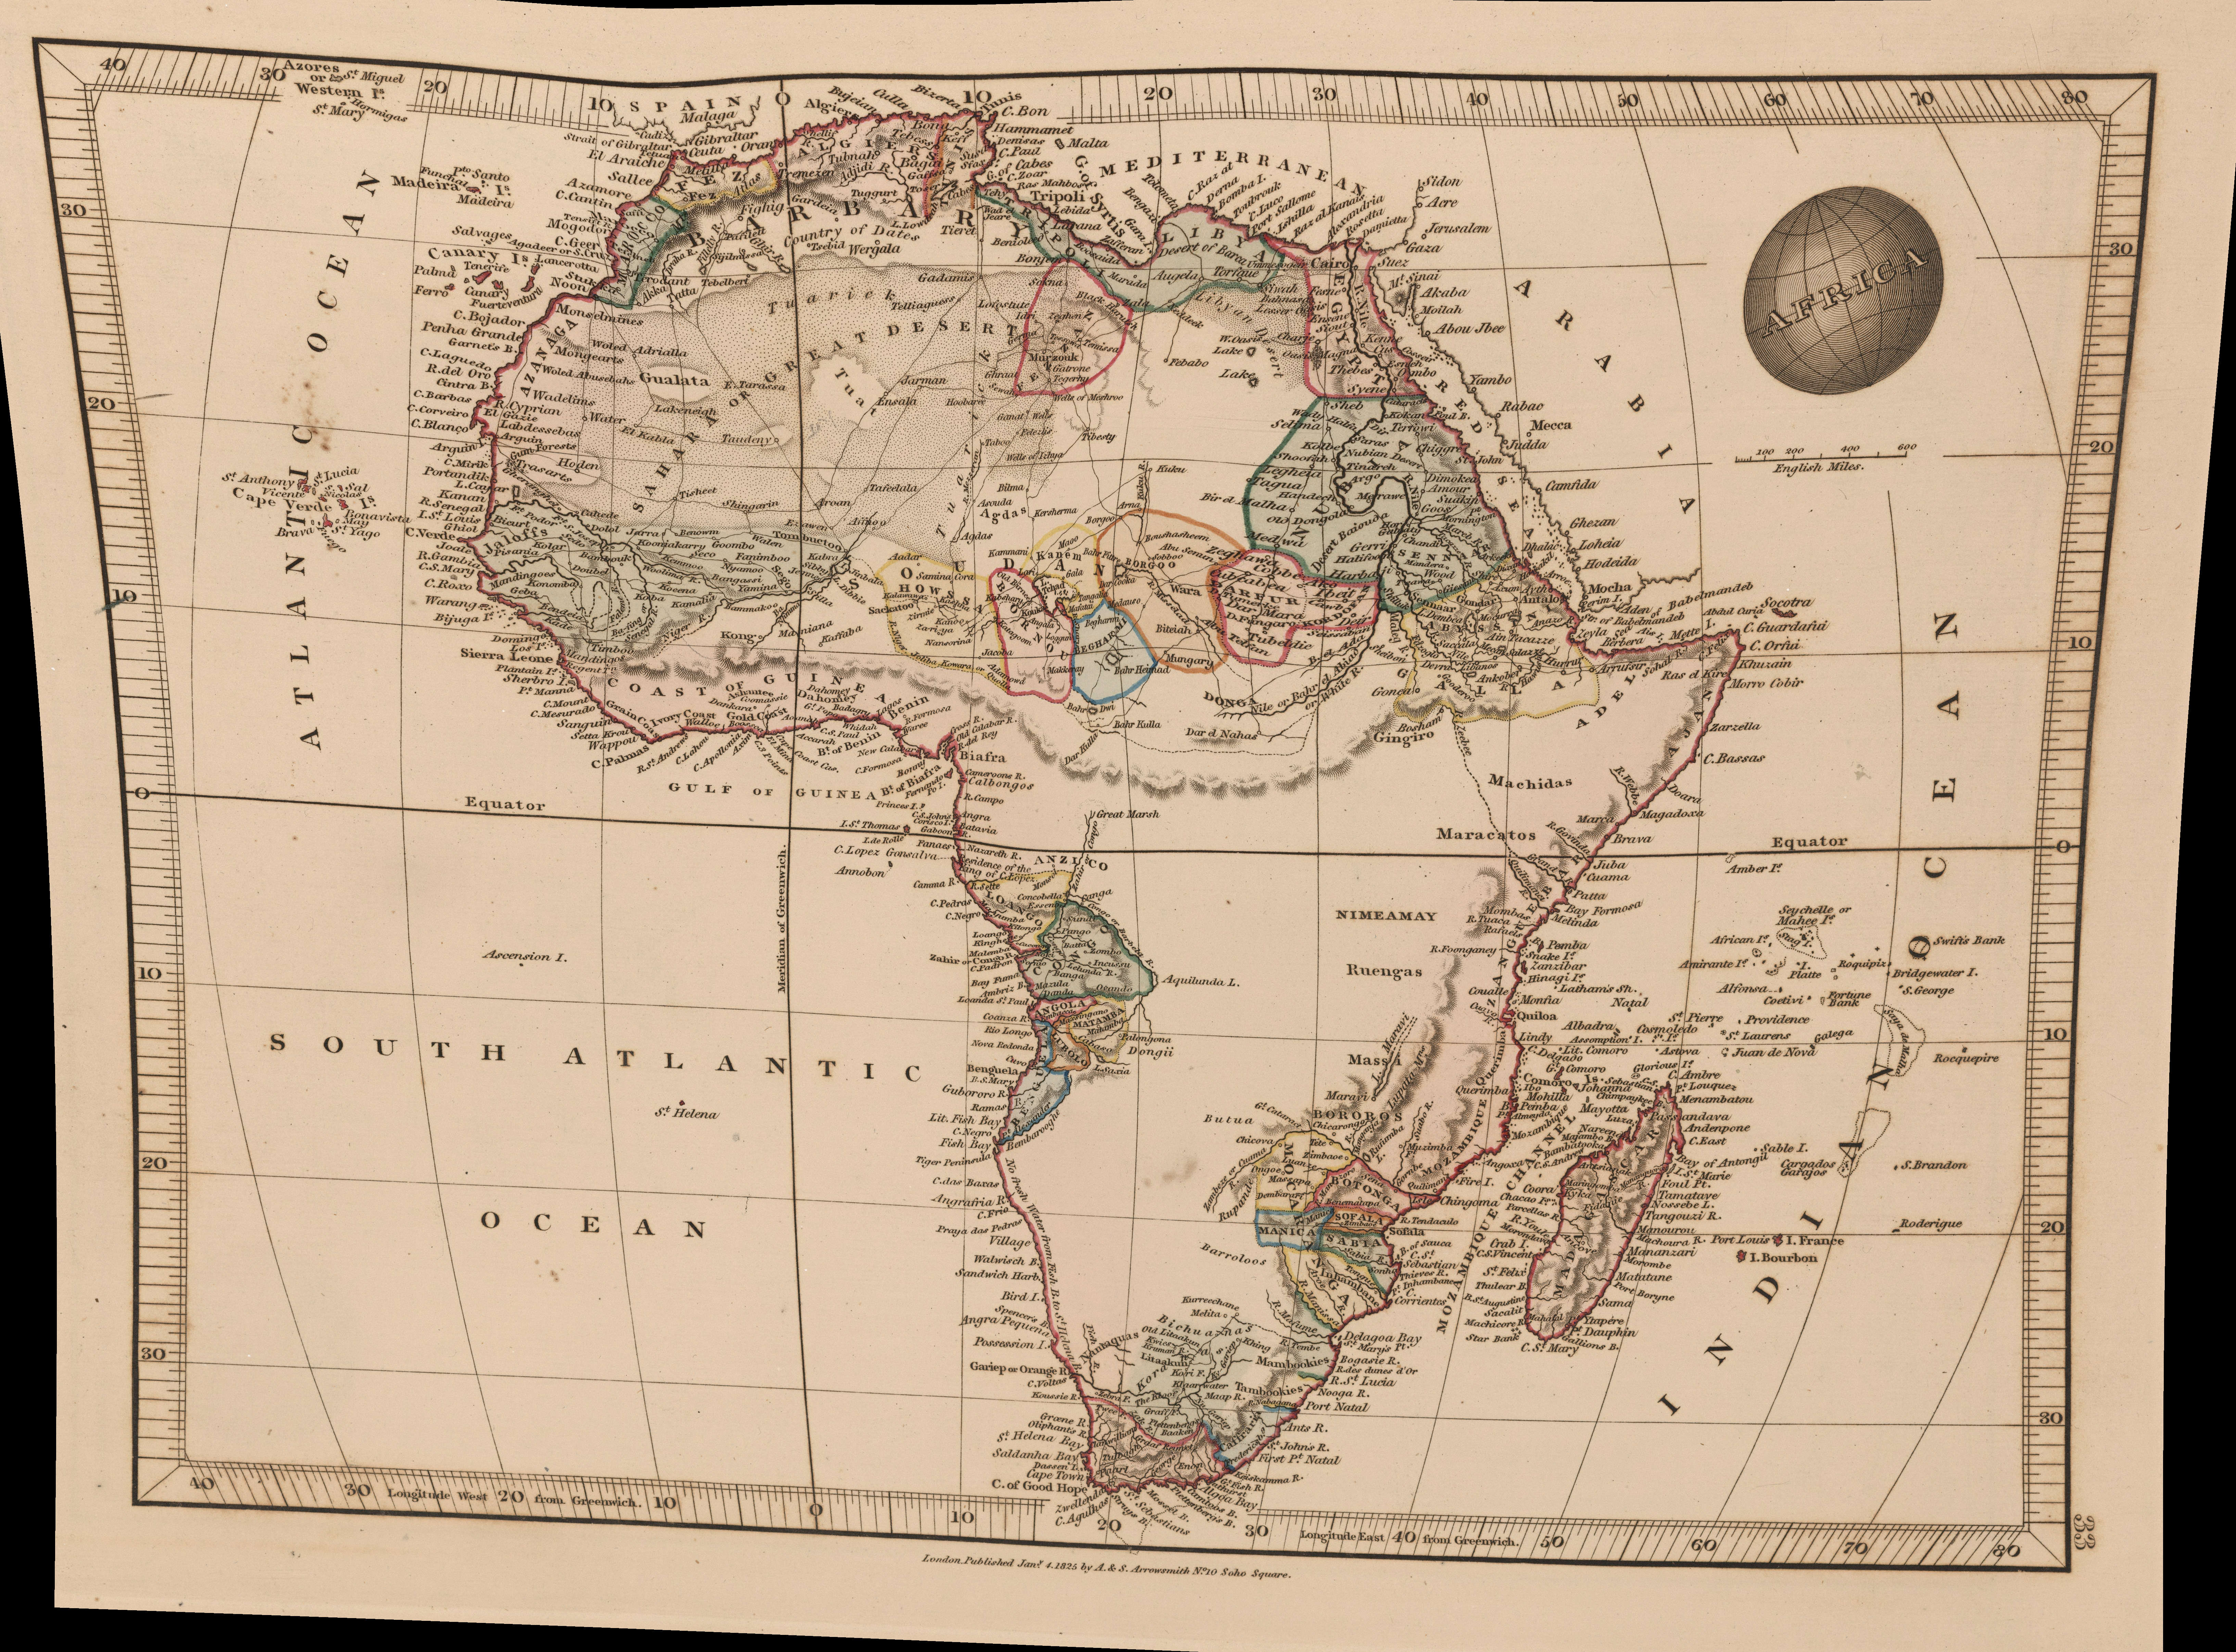
\includegraphics[width=0.8\linewidth]{img/Arrowsmith.jpg}
	\caption{Example of georeferenced map}%
	\label{Arrowsmith}
\end{figure}

%\begin{multicols}{2}

\subsection{The mountains of Kong} \label{The mountains of Kong}

The accuracy of the historical maps used to create the polygons of the Geo-ISD
is a natural concern. Who typically drew these maps? Based on what sources? For
what purposes? And with what level of technical accuracy? 

Most of the maps from the David Rumsey project were from atlases published
for commercial purposes by individuals or small publishing companies
specializing in this type of publications. Most are from English or American
atlases, but French, Italian, German and other sources are included as well. The
maps were based on a combination of existing maps updated with `the latest
sources' (a fact frequently boasted in the title of the atlas), which for the
majority of the period meant explorers or geographers on missions from their
respective geographical societies.\footnote{Later maps additionally draw on the
	work of military surveyors, but as far as I have been able to tell the
majority are still based primarily on the work of explorers and past maps.} In
the words of \citet[47-48]{Stone1995}: `Cartography in Africa [in the 19th
century] is still a mix of measurement, less accurate observations, word of
mouth, previous maps and sources, educated guesses and pure conjecture.
Nevertheless a distinct improvement on the maps of previous periods.'. Because
of this, I expect two types of errors: errors resulting from measurement, and
bias resulting from misconceptions (deliberate or not) of what constituted the
borders of a polity at the time. I also expect errors to be replicated by other
maps, before eventually being corrected. One example of this is the nonexistent
Mountains of Kong, which can be seen in Figure \ref{Arrowsmith} as the mountain
range stretching across most of the continent from East to West. These mountains
were replicated for the better part of the nineteenth century before
eventually being wiped from the map \citep{Bassett_1991}.

While the quote above might lead one to expect considerable measurement error,
by my estimate this error only amounts to 36.9km on average for the shapes
included in the GeoISD. This estimate is based on the estimated mean distance of
the coastline in the maps to the real coastline, along the borders of the states
that were traced. This captures measurement error explicitly, because regardless
of where states did or did not extend their control, the coastline in the map
should line up with the real coastline. This means that there are often multiple
estimates for each map, reflecting how the accuracy is better in some places
than in others. If this difference was above 100km, the maps were deemed too
inaccurate and excluded from the sample. Error estimates for states that lay
inland were not included, because consistently matching features from the maps
to real geographical features was not feasible other than when using the
coastline, which provides a visible line of comparison. Additionally, this type
of error only adds noise, because it is equally likely to err in one direction
or the other. Thus it should not affect coefficient estimates, but could
potentially affect standard error estimates.

Although I have not been able to find sources discussing specifically how
cartographers determined the borders of different polities, it is probable that
they in large part relied on local verbal sources (word of mouth). An example of
this can be glimpsed in the exchange where the explorer Mungo Park effectively
dubbed the mountains of Kong.\footnote{`I gained the summit of a hill, from
	whence I had an extensive view of the country. Towards the south-east,
	appeared some very distant mountains, which I had formerly seen from an
	eminence near Marraboo, where the people informed me, that these
	mountains were situated in a large and powerful kingdom called Kong; the
sovereign of which could raise a much greater army than the King of Bambarra.'
\citep[CHAPTER XVIII]{ParkMungo2015Titi}.} Or from when expeditions such as
Park's were escorted by representatives of the rulers of the various polities
they passed through, until reaching \textit{frontier towns}, where they would be
met by representative of the next ruler \citep{ParkMungo2015Titi}. In the maps
resulting from such encounters, both their sources as well as the cartographers
themselves could have introduced bias to the resulting maps. Sources were likely
to be rulers or their representatives, with incentives for aggrandisement. The
explorers and cartographers on their part represented European rulers with an
eye toward colonial expansion. It less clear how this would affect the resulting
borders drawn. One potential bias would be to exaggerate the domains of your own
governments prospective colonies, and vice versa. Another possibility is that
colonial cartographers under reported state sizes to declare `terra nullius'.
However, I did not observe any systematic differences between the maps based on
their nationality.\footnote{If drawing borders was driven by colonial ambitions,
there should be observable differences between the different colonial powers in
line with their differing colonial ambitions.} In fact, their colonial ambitions
could just as easily have promoted accuracy, as any potential military
expedition would benefit from accurate information \citep{Bassett_1994}.

\subsection{A topographical representation of the state} 
\label{A topographical representation of the state}

At the very least there should be heterogeneity in the conceptualization of
territoriality. What determines where a given source (or the cartographer in the
second instance) draws the borders of a polity, or how this would vary with
their respective conceptualization of states, polities and ethnic groups, is
impossible do determine. However, thanks to (usually) having multiple maps for
each state, the variation can be leveraged to create a measure of the
\textit{degree} to which a state had a presence in a given area over the time
period as a whole. When maps disagreed on where the various borders were, I
interpret this as either true variation across time, or as an indication of the
ambiguity of where a given state had nominal or real control. In the areas where
all the maps agree, one could be quite sure that the given polity had real
presence.  While in areas where only one map indicated that the state was
present, this could either be wrong, an indication of nominal as opposed to more
real presence or some other form of limited presence. The coding process of
looking at hundreds of maps strengthened this initial intuition, and the
resulting figures of state presence drawn from the complete data lends it
further credence. Figure \ref{nigeria} demonstrates how the estimate of
pre-colonial state presence captures a topographical measure. In the figure the
Northern states of Sokoto (North-West), Borno (North-East) and Adamawa (East)
are clearly distinguishable, while the Southern states (primarily the Benin
kingdom, neighbouring Dahomey and the multiple Yoruba states) have a weaker
presence and blend more together. The reason for the lower state presence in the
South is in part that these kingdoms were younger, or lasted shorter, than the
Northern states, and that they conformed to fewer mapmakers and histories
conceptualisation of `state'. Furthermore, the figure demonstrates how the
presence of the Northern states gradually fades away from the center. In some
places it fades gradually, as the Sokoto Caliphate to the South. This presumably
reflects the temporary high water mark of its southward expansion, before being
repulsed by the Yoruba kingdom of Ibadan. Other places state presence fades
rapidly, as Borno to the North, where its borders meet Lake Chad.

%\end{multicols}

\begin{figure}[htpb]
	\centering
	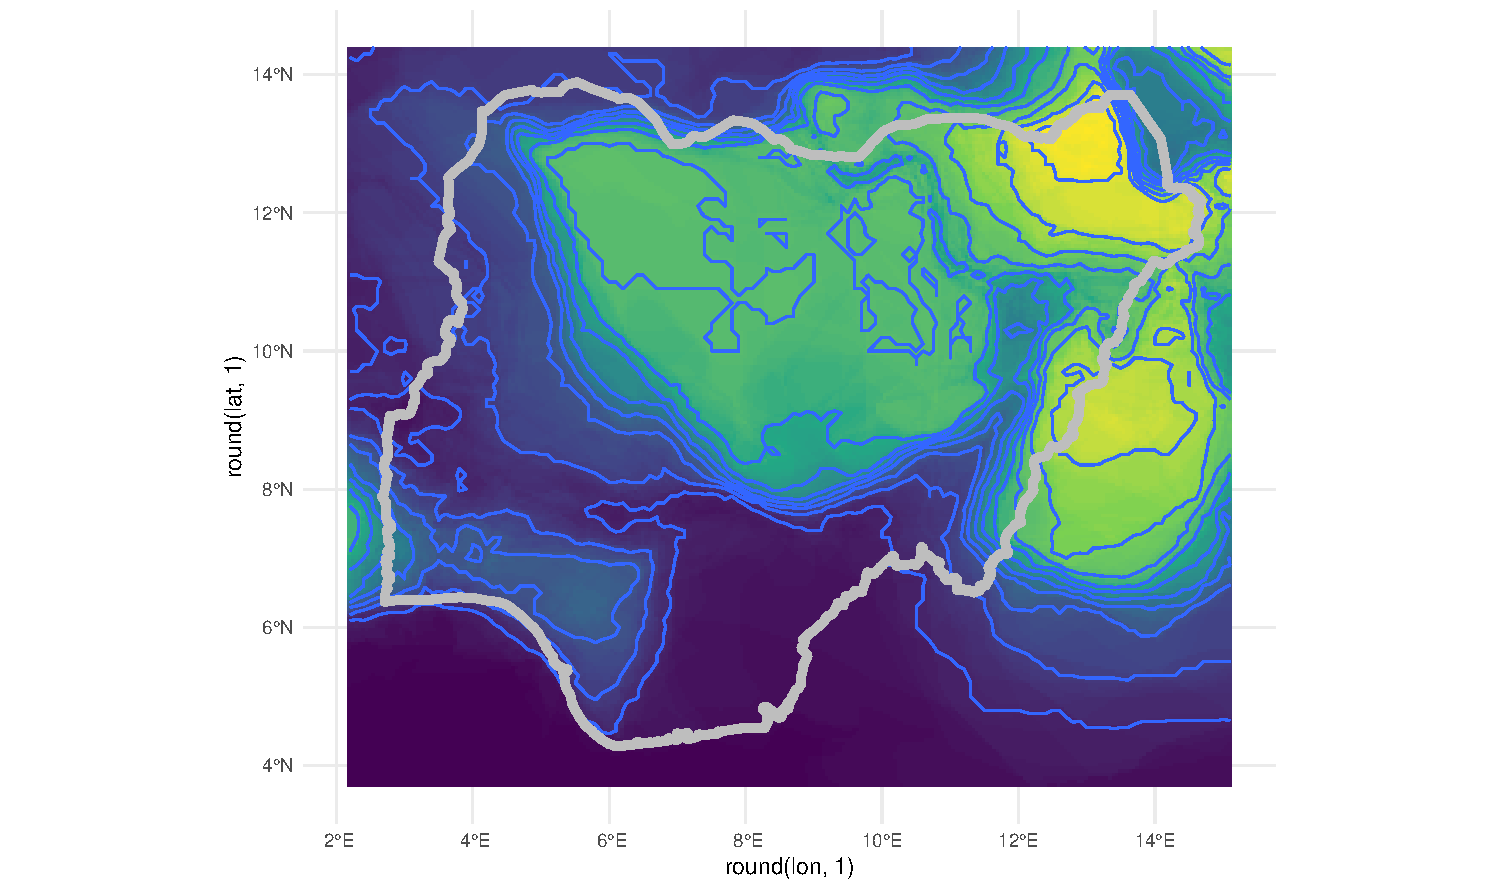
\includegraphics[width=\textwidth,keepaspectratio]{../R/Output/nigeria.pdf}
	\caption{Pre-colonial state presence in Nigeria (1800-1914).}
	\label{nigeria}
\end{figure}

%\begin{multicols}{2}

% To counter balance some of the potential bias in the historically
% contemporaneous maps a number of maps from historical atlases were included.
% These are works compiled by historians with both the accumulated knowledge of
% history and modern instruments of cartography at their disposal. These sources
% should be able to reduce problems of the historically contemporaneous maps, such
% as word of mouth sources exaggerating the extent of polities.\footnote{Although
% 	they should also be more accurate in terms measurement error, I found
% that this was not always the case. For example \citep{Kasule1998} completely
% misplaces Wadai, putting the capital of Wara (and thus the rest of the polity
% with it) at least 200km North West of its actual position.} The historical
% atlases were scanned, then georeferenced and polities traced in the same manner
% as the pre-colonial states in the historically contemporaneous maps. The
% historical atlases frequently depicted the borders of states over a period of
% years in a single map. In these cases the resulting state shapes were duplicated
% for each year in the period. This has the benefit of placing a larger emphasis
% on the historical atlases, at the cost of being more static.\footnote{Implicitly
% assuming constant borders, and in the absence of other sources implying uniform
% control across territory.} Figure \ref{atlasmaps} in the appendix lists the
% historical atlases used in the Geo-ISD.

The resulting data can be compiled in different ways, to provide different
insights. For the analysis in this paper I rely on a measure of `state
presence', similar in concept to that of `state history' introduced by
\citet{Depetris-Chauvin2016}.\footnote{The main difference between these
	measures is that `state history' is measured in 2 by 2 decimal degree
	grid cells, only includes Sub Saharan Africa, includes fewer states
	despite going further back in time, usually only includes one shape per
state, which implies static borders and uniform presence throughout the
territory.} I measure `state presence' the as number of state-shape-years that
indicate that a state was present in a cell, counting only those of the state
most often present in that cell. If a cell contains 40 shapes of the Sokoto
Caliphate and 7 shapes of Borno, only the Sokoto shapes are counted. Including
the Borno shapes would risk over counting, as it most likely does not represent
additional state presence, but rather overlapping or contested sovereignty.

%\end{multicols}

\begin{figure}[htpb]
	\centering
	%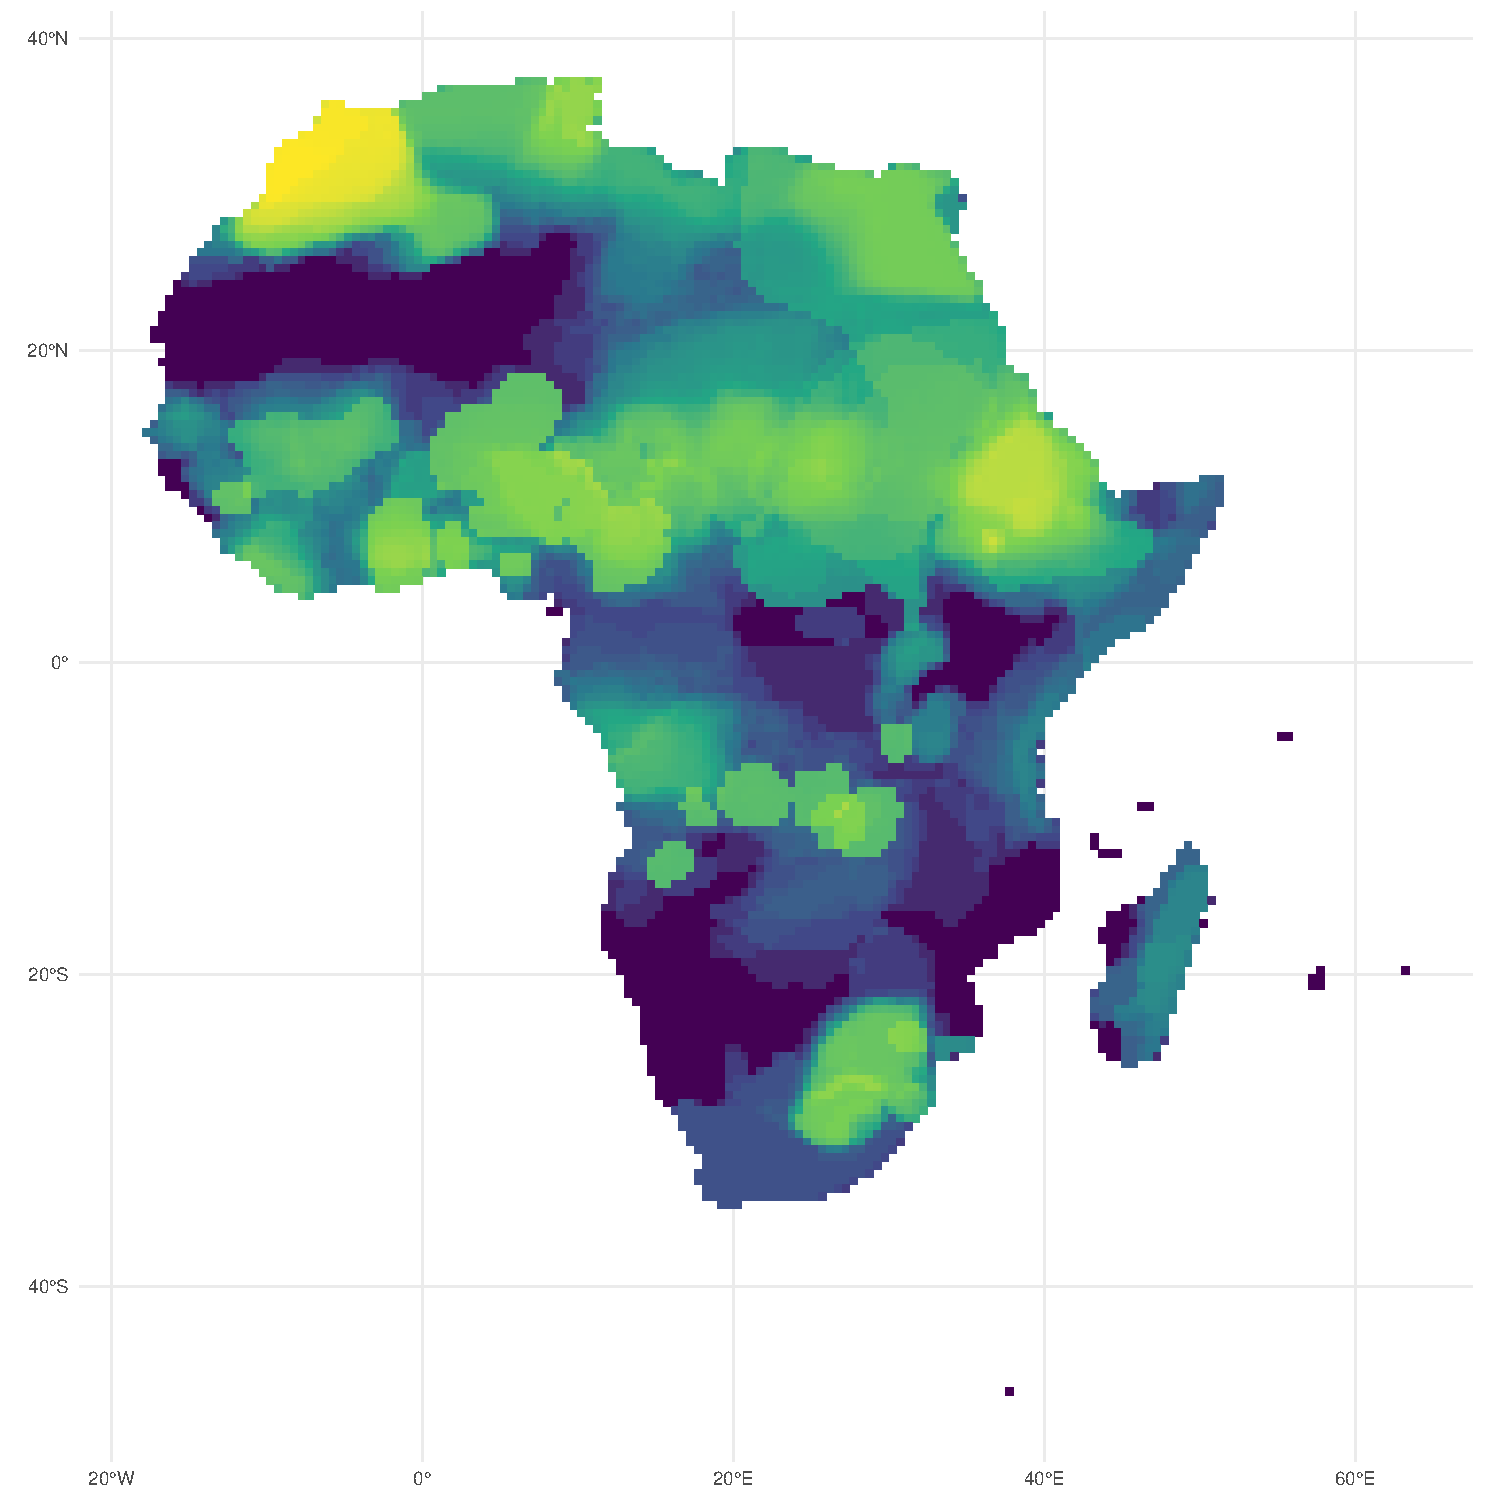
\includegraphics[width=0.8\linewidth]{../Rplot_ln_sp_int.pdf}
	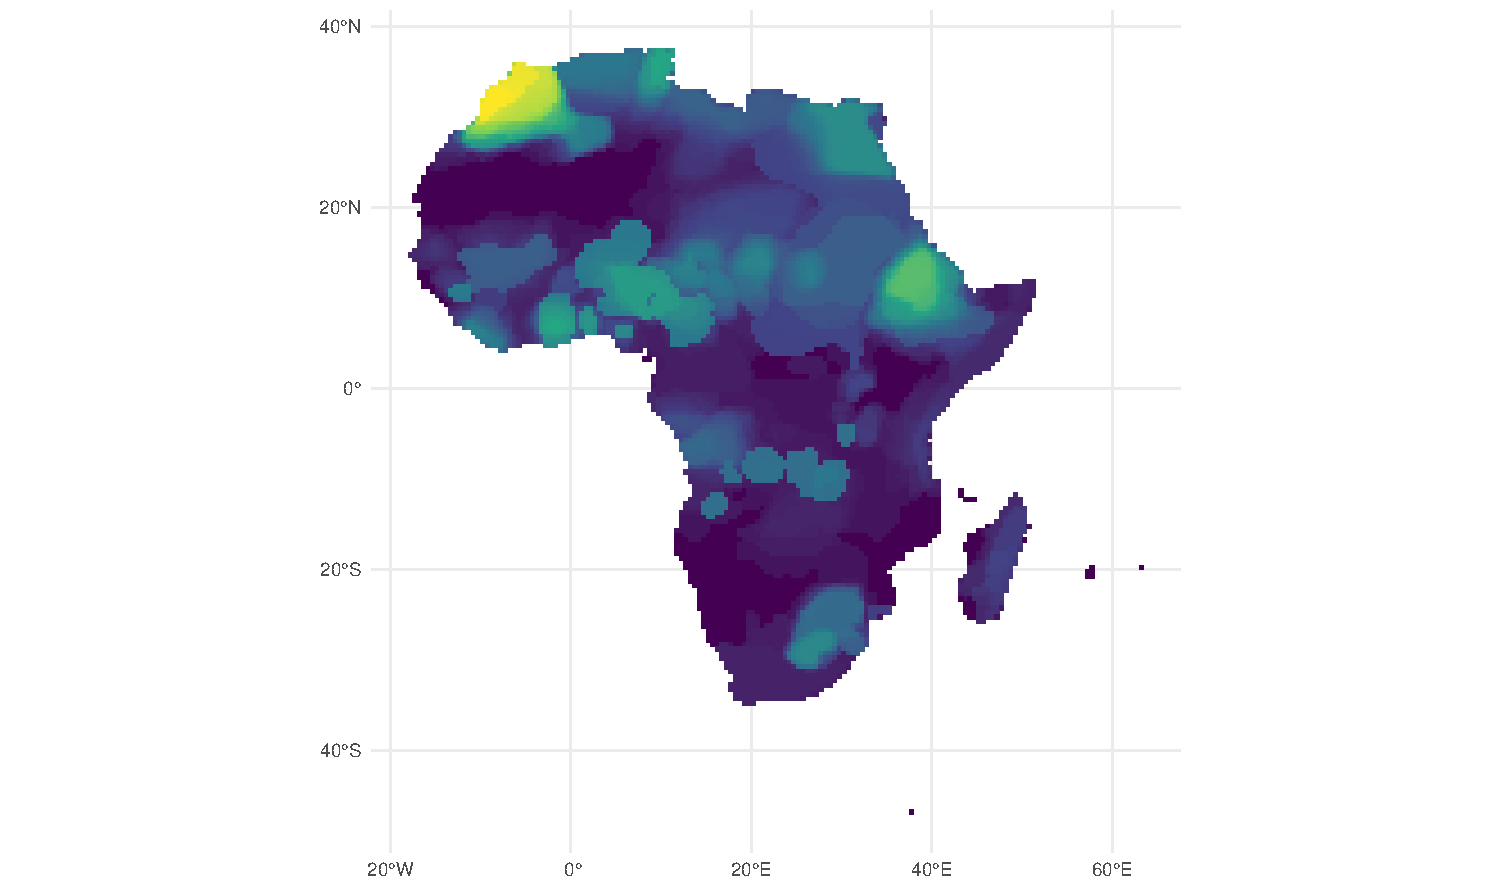
\includegraphics[width=\linewidth]{../R/Output/sqrtSpAll.pdf}
	\caption{State presence (sqrt transformed) with interpolated years based
	on historical atlases.}
	\label{Sp_i}
\end{figure}

%\begin{multicols}{2}

\section{Research design} \label{Research design}

\subsection{Dependent variable} \label{Dependent variable}

The units of analysis are PRIO 0.5 by 0.5 decimal degree grid cells with a
non-zero population density in 1600,\footnote{This primarily excludes the Sahara
and Kalahari deserts.} which equals about 55 by 55km at the equator
\citep{Tollefsen2012}. Due to the explanatory variable being time-invariant, the
analysis is a cross section. The main dependent variable is state based conflict
related fatalities per grid cell over the period 1989-2020, from the GED project
\citep{Sundberg2013}. This is a measure of the overall level of conflict in the
post cold war period. The start date of 1989 was dictated by availability rather
than chosen by design, as it likely biases against finding results (positive or
negative), because the mechanisms discussed in the theory section should have a
more powerful effect closer to independence and would fade in relative
importance with the passing of time.

As an alternative to combat related fatalities, I also ran models using the
count of state based conflict events. This captures much of the same general
level of conflict during the period as the fatalities measure does, but the
focus is slightly different. Fatalities more so captures the severity of
conflict, whereas the number of conflict events more so captures the frequency
of conflict. This would be the difference between few, or short, but highly
lethal conflicts, versus lengthy conflict of relatively low intensity, or
recurring conflicts. I do not expect there to be a substantial difference in the
results from these measures based on the theory presented above.

% While some of the theoretical mechanisms discussed above might be more closely
% related to a specific type of state-based conflict, such as wars of secession,
% these are difficult to separate entirely. That is, they are unlikely to manifest
% \textit{exclusively} as a specific type. This does not mean that the choice of
% dependent variable biases in favor or finding a relationship. In fact
% \citet{Wishman2021a} finds that pre-colonial state presence has a negative
% effect on communal violence events. 

\subsection{Independent variables} \label{Independent variable}

% However, only the state that has the most presence overall in that grid cell is
% included, so as to avoid over counting in cases of overlap (contested
% sovereignty) or when territory has changed hands. This measure has the benefit
% of including more data, which allows for the approximation of relative degrees
% of state presence by one state in any year, as described in the data section
% above. At the same time it avoids over counting state presence where there were
% overlaps in sovereignty or changes in who controlled the territory. 

Because I do not expect the relationship between pre-colonial state presence and
civil conflict to be linear, and because the data is heavily skewed, the
variable is square root transformed. While log transformation is more often
employed in the previous literature, the variable contains zeros. This is
usually solved by adding a constant to all values. However, this could
potentially introduce bias, and complicates the interpretation of the results
\citep{Ekwaru_2018}. I therefore present the more conservative approach of using
a square root transformation for the main models.\footnote{In addition to the
	square root transformed version of the main independent variable, I also
	ran models using the more common log transformation. The results
remained substantially the same, but with larger effect sizes.} This has the
benefit of not having to add a constant, but produces a less evenly distributed
variable. 

The main explanatory variable is an interaction between pre-colonial state
presence (square root transformed) and distance to capital (log transformed).
The theoretical expectation is that pre-colonial state presence is conflict
reducing in areas close to the post independence capital, and conflict inducing
in more remote areas. In other words that the effect of pre-colonial state
presence is moderated by distance to capital. Distance to capital is log
transformed because I do not anticipate a linear effect. Because the variable is
measured by distance from the center of each grid cell to a point indicating the
capital, there are no zeros and log transformation can be done without adding a
constant. Distance to capital is sourced from the PRIO-grid data set, but
originally from \citet{Weidmann2010a}.

As a further robustness check I also ran models using a measure of state
presence that sums if there ware any maps that included a state in a
grid-cell-year (as a sum of yearly dummies). In other words, this could be at
most 214, and is more a measure of the maximum \textit{extent} of state
presence, and is less accurate in terms of variations in depth. The benefit of
this measure is that it avoids some of the potential over representation of
countries frequently mapped by Europeans, such as the North African states (due
to proximity). As with the main measure of state presence, only the shapes of
the state that was most present in that grid cell throughout the sample period
were traced. Results remain substantially the same for all specifications.

\subsection{Controls} \label{Controls}

Because the treatment variable in this case predates the outcome by a long
period of time, there is a substantial risk of introducing post treatment bias
when including control variables. In choosing which control variables to
include, I try to balanced a trade off between potential post treatment bias
and omitted variable bias. 

Mountains facilitate early state formation by providing protection and limiting the
exit options of sedentary farmers \citep{Carneiro1988}. Mountainous terrain has
also been linked with civil conflict by providing shelter for rebel groups
\citep{Hegre2006}, although this relationship is debated \citep{Buhaug2002}. The
data is from the PRIO-grid data set, but originally from \citet{Blyth2002}, and
measures the percentage of the cell with mountainous terrain based on elevation,
slope and local elevation range.

Water is essential for state formation. States typically formed either around
coastal cities, close to navigable rivers or by the shores of great lakes.
People still tend to live next to a source of water, thus this acts as a proxy
for population density, and fighting usually happens where there are (at least
some) people. The data on water as a percentage of the grid surface is from the
PRIO-grid data set, but originally from the European Space Agency
\citep{Bontemps2009}.

Distance to the coast could affect both state presence and conflict in a number
of ways. First, as stated above, states were more likely form along the coast as
it connected cities and people. A special case for Africa is also the existence
of slave raiding/trading states that formed along the eastern and western coasts
of the continent. These state's raison d'être was raiding slaves from tribes and
peoples inland and selling them to coastal traders (European in the West and
Arab in the east). \citet{Nunn2008} argues that this state of affairs left
legacies of mistrust and antagonism, which has resulted in increased levels of
current day conflict. Distance to the coast could also be related to the measure
of state presence through the fact that our measure is based on European
observations (maps), which undoubtedly had better coverage along the coast,
especially for the earlier periods. Distance to the coast could further be
related to conflict through lower levels of economic development inland. The
distance to coast data is from \citet{Wessel1996}. The variable was log
transformed to account for a non-linear relationship.

As with water, barren terrain could be a (negative) pre-condition for state
building as well as proxy for later population densities, and thus could
correlate with both state presence and levels of conflict. The data is from
\citet{Bontemps2009}.

The states of North Africa are overrepresented in the Geo-ISD data, due to the
geographical proximity, and the accompanying historical familiarity to European
map makers. This affects Morocco most particularly, as can be seen in Figure
\ref{Sp_i}. The reason this affects Morocco in particular is that the remaining
North African states were under Ottoman suzerainty for much of the period. If
North Africa is also more or less conflict prone than the rest of Africa on
average, the inflated values of state presence would bias the estimated
coefficients. Accordingly, I included a dummy variable for the region of North
Africa.

Population density is added due to the theoretical expectation that it could be
a confounding variable. There are few accurate measures of population densities
that predate most of the states in the Geo-ISD. The best available estimates
come from the HYDE project \citep{Goldewijk2016}, and I use the estimates from
1600.

Distance to international boundaries could be related to state presence because,
despite their reputation, African borders were not drawn completely at random
(or along meridian lines). For example, the boundary between northern Nigeria and
Niger were based on the extent of the Sokoto Caliphate and the neighboring
Kanem-Bornu (or just Bornu) empire \citep{HiribarrenVincent2017AHoB}. Proximity
to an international boundary has also been found to predict conflict
\citep{Buhaug2002}. I use the measure included in the PRIO grid data, which is
originally from \citet{Weidmann2010a}.


\subsection{Modelling} \label{Modelling}

To account for the potential post treatment bias (vis-a-vis potential omitted
variable bias) controls were added step wise with increasing potential for post
treatment bias. The baseline model only includes geographic variables, which
should safely pre-date any states and thus be free of post-treatment bias.
Subsequent models add controls according to likelihood of introducing post
treatment bias.

To account for the dependent variable being count data (count of deaths
(fatalities) and count of conflict events (state based)) all model
specifications reported below are negative binomial regressions or zero inflated
negative binomial regressions. A fitness test for whether negative binomial or
Poisson regression is most appropriate, was conducted and confirmed that
negative binomial produced a better fit than Poisson.

The dependent variable contains excess zeros (8937 zeros relative to 100 counts
of 1 fatality, the second most frequent outcome). Additionally, I cannot be sure
that the main independent variable affects the likelihood of there being any
fatalities in a cell (or if it remains a zero), the same way it might influence
the severity of conflict once a cell has seen at least one fatality. I therefore
employ a zero inflated negative binomial model. The first step of this two step
approach is a logit that models the likelihood that a cell experiences conflict.
I used the same set of controls as I do not expect any of them to exclusively
affect conflict severity, nor do I expect their relation to the main independent
variable to be substantially different for an onset model. The second step is a
negative binomial estimation of conflict severity, or the number of
fatalities/events in a cell that has seen at least one fatality/event.

Given what is known about spatial diffusion of conflict, there is reason to
suspect some spatial autocorrelation. However, controlling for this would
introduce a source of post treatment bias. [why?] Nevertheless, as an additional
robustness check I ran some models with queen pattern spatial lags. Most of
these models did not converge, but those that did remained substantially similar
to the main models.

\subsection{Testing the mechanism} \label{Testing the mechanism}

Testing the proposed mechanisms explicitly would require data on where elite
networks and institutions have survived from pre-colonial states, or data on
rebel groups use of symbols invoking past statehood. Collecting such data lies
outside the scope of this paper. Fortunately, the differences in the approach to
colonial governance between Britain and France could provide a proxy for the
elite networks and institutions mechanisms. France generally sought (more
successfully in some cases than in others) to fully incorporate and rule their
colonies directly, dismantling existing institutions and avoiding a reliance on
native administrators \citep{Blanton_2001}. Britain, on the other hand, pursued
a strategy of indirect rule, preferring to leave local rulers to administer
their own territories, and relying on their own institutions to do so
\citep{Blanton_2001}. Former British colonies should therefore be more likely to
have preserved the elite networks and institutions that could be used to
mobilize against the state. I therefor ran all the models including controls for
former French and British colonies. [Theory implies interaction, but three-way
interactions are a impossible to interpret, perhaps better to re-run main models
on French and British sub samples.] In these models, the North Africa control had
to be dropped because most of North Africa were French colonies at some point
and models would not converge with both included. 

[Territorial disputes far from the capital and government disputes close to
capital?]

\section{Results} \label{Results}

Despite the data on conflict starting nearly three decades after most of Africa
achieved independence (at which point the effects of pre-colonial state presence
on conflict should be most pronounced), there is a significant
and positive direct effect of state presence on conflict (.11, SE = .01 and .10,
SE = .01 in the main models). This effect is robust and stable across all models
(see Table \ref{statebaseddeaths} and Table \ref{state_based}). All controls
have the expected signs except distance to coast in Table \ref{state_based},
using state based conflict events as the dependent variable. However, the
coefficient indicates a substantially negligible effect, and the statistical
significance might be more a reflection of the large number of observations
(9492) rather than any underlying causality. The second model in Table
\ref{statebaseddeaths} indicates that North Africa has experienced more conflict
fatalities than the rest of Africa comparatively. However, this effect becomes
smaller and is no longer significant at the $ p < .01 $ level after controlling
for population density in 1600, suggesting at least part of the effect could be
due to higher levels of population density.

However, the results of the interaction models reveal a more nuanced picture. As
seen in Table \ref{interaction_statebaseddeaths} and Table
\ref{interaction_state_based}, when adding the interaction term between state
presence and distance to capital, state presence has a conflict reducing effect,
albeit a non-significant effect in the fatalities models. All control variables
behave as expected, and similarly as in the non interaction models.
Unsurprisingly, distance to capital (log) is negative, as there is generally
less conflict close to capital cities. The interaction term is significant
and positive across all model specifications, in line with the theoretical
expectations. 

In terms of substantial effects Figure \ref{deaths_zinb}, which models the
predictions of the second stage ZINB model included in Table \ref{zinb},
provides a more intuitive interpretation of the interaction between state
presence and how it affects the severity state based conflict. State presence is
negatively correlated with both conflict measures close to the capital, but
becomes positive and significant further away from the capital. This is in line
with an interpretation that state presence can be conflict reducing in those
areas where it makes a territory less artificial, by providing institutions and
elite networks on which to build a state. In cases where there is no state
presence in capital areas, the model predicts an additional 406 fatalities from
state based conflict. The effect drops rapidly as state presence increases. On
the other hand, in areas with no experience of statehood that are far from the
capital, the model predicts almost no additional fatalities (similar to high
levels of state presence in/around the capital). However, as state presence
increases, so does predicted fatalities. For a mean plus one standard deviations
level of pre-colonial state presence of 138, the main model predicts an
additional 250+ [find exact]
fatalities. While this is not a test of the specific mechanisms outlined in the
theory section, the results do indicate that symbols, elite networks or
some other legacy of pre-colonial statehood raises the scope of conflict
in areas remote to the capital.

%\end{multicols}

\begin{figure}[htpb]
	\centering
	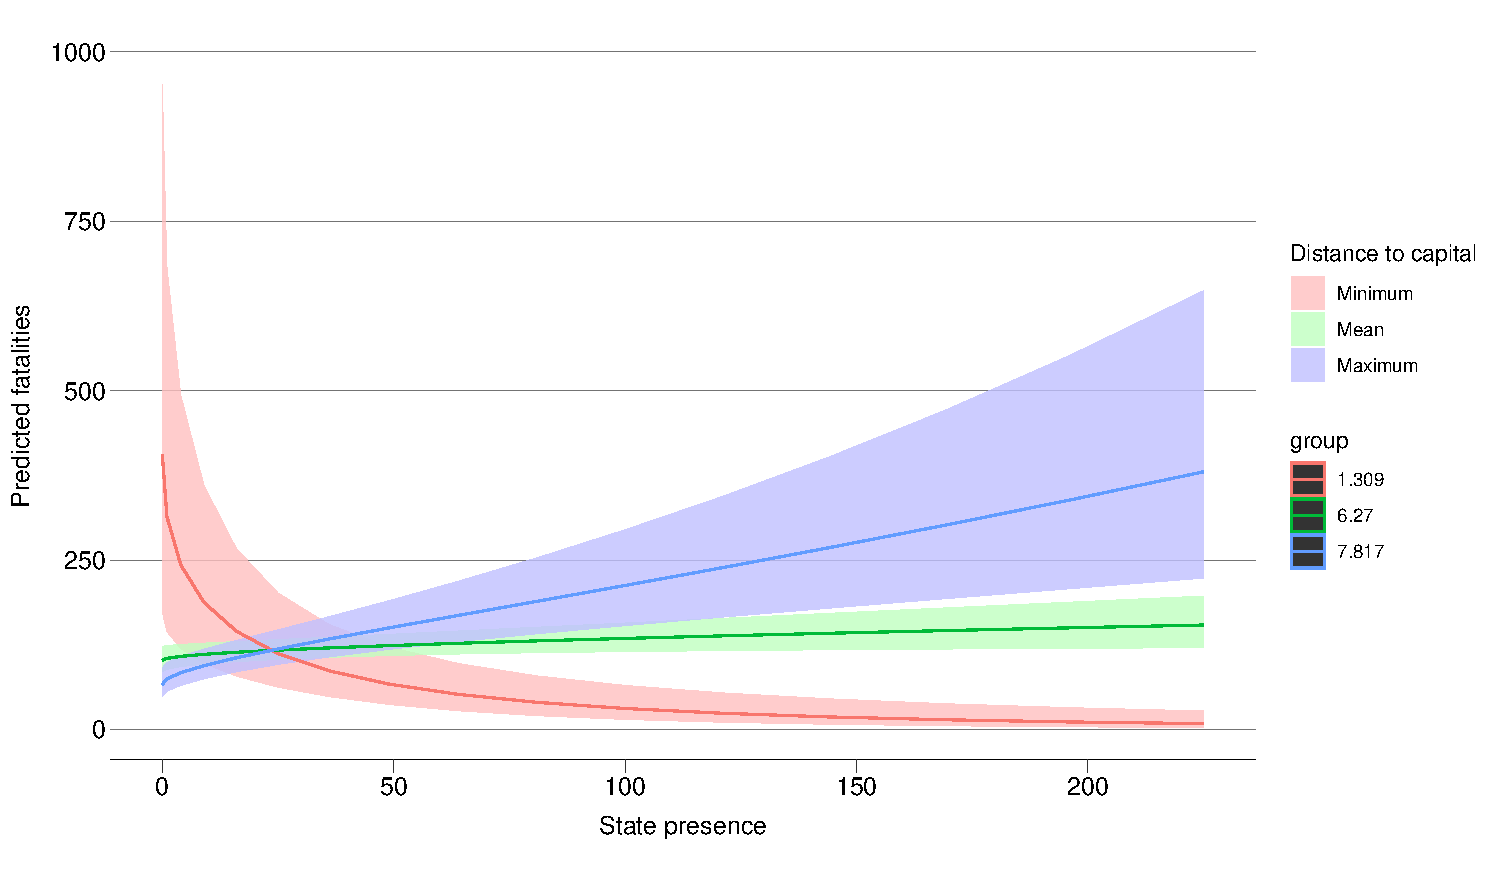
\includegraphics[width=\linewidth]{"../R/Output/zinbplot.pdf"}
	\caption{}
	\label{deaths_zinb}
\end{figure}

%\begin{multicols}{2}

The results of the models including controls for French and British colonies
(see Table \ref{zinb}) are interesting in that the predicted increase in conflict
severity in capital areas without prior experience of statehood is at 991
additional fatalities. The signs of the colonial controls are as
expected. However, the conflict inducing effect of being a former British
colony is only significant on conflict onset (the first stage logit
model). Similarly, the conflict reducing effect of being a former French colony
is only significant in terms of reducing conflict severity (second stage
negative binomial count model). These results can not be interpreted with any
certainty, but do perhaps suggest that French style governance left stronger
central government that were better equipped to limit the scope of conflicts,
while the British tradition of indirect rule left a larger number of potential
rivals to the central government. [This needs to be adjusted according to
results of sub sample model results] [Results of territorial and governmental
conflict]

\subsection{Alternative explanations} \label{Alternative explanations}

An alternative interpretation of the results could be that this is a
story of more coherent ethnic groups being more likely to be associated with
states, and more likely to (perhaps better able to) challenge the government
when situated far from the capital. However, getting closer to the real
causality requires untangling, for each case, if a given conflict is related to
an ethnic group's ties to a pre-colonial state or not. This lies outside the
scope of this paper, if it is even possible.

Another interpretation that is not controlled for in this paper is the
possibility that past conflict drives both state creation and current conflict.
However, data on past conflict is meager, especially so for Africa. To my
knowledge the \citet{Brecke1999} data set is the most complete. Even so, it
relies on written histories of which there is little for pre-colonial
sub-Saharan Africa. What is worse, the missing will be considerably biased
because kings and states are far more likely to chronicle their warfare in the
form of written records. [Icing: use data Charles got for the other data]

\section{Conclusion} \label{Conclusion}

Drawing on the emerging literature on pre-colonial states \citep{Paine2019,
Depetris-Chauvin2016}, institutions \citep{Wig2016, Englebert2002,
Michalopoulos2018} and civil conflict, and on newly compiled data, this paper
re-examined the relationship between pre-colonial states and civil conflict. I
find a general conflict inducing effect of pre-colonial state presence on local
levels of state-based conflict. However, I also find support for a conflict
reducing effect of pre-colonial state presence, but this is conditioned on the
relationship between the pre-colonial state(s) and the post-independence state,
as [proxied] by the distance to the post-independence capital. On the other
hand, I find strong evidence for a conflict inducing effect, particularly in
areas far from the post-independence capital. These results are robust to
alternative measurements and model specifications.

These findings have a few important implications. First, they demonstrate that
pre-colonial states can be a blessing or a curse depending on whether they form
the basis of the modern state or a point of opposition to it. Second, that local
political histories matter, and should be taken into consideration by
policymakers and scholars alike. Finally, these results suggests that wherever
colonizers left novel constellations of pre-existing polities, they unknowingly
sowed the seeds of future conflict. More research using global data is needed to
test whether general trends for Africa hold outside that continent as well.
[Somewhere in this section fit in the prediction that there is potential for
violence in places where the central government has not yet extended its reach
into areas with high degree of pre-colonial state presence, most notably in
Puntland, Somalia.]

%\end{multicols}

\pagebreak

\bibliographystyle{apalike}
\bibliography{../lib.bib}

\pagebreak
\section*{Appendix}


% Table created by stargazer v.5.2.3 by Marek Hlavac, Social Policy Institute. E-mail: marek.hlavac at gmail.com
% Date and time: Thu, Apr 28, 2022 - 03:16:56 PM
% Requires LaTeX packages: rotating 
\begin{sidewaystable}[!htbp] \centering 
  \caption{Summary Statistics} 
  \label{summarystats} 
\begin{tabular}{@{\extracolsep{1pt}}lccccc} 
\\[-1.8ex]\hline 
\hline \\[-1.8ex] 
Statistic & \multicolumn{1}{c}{N} & \multicolumn{1}{c}{Mean} & \multicolumn{1}{c}{St. Dev.} & \multicolumn{1}{c}{Min} & \multicolumn{1}{c}{Max} \\ 
\hline \\[-1.8ex] 
Fatalities & 10,652 & 883.7 & 10,710.9 & 0 & 615,886 \\ 
Conflict events & 10,652 & 4.0 & 38.0 & 0 & 1,773 \\ 
State presence & 10,652 & 50.2 & 88.1 & 0 & 629 \\ 
Distance to boundary & 10,652 & 138.1 & 122.6 & 0.003 & 668.0 \\ 
Distance to capital & 10,652 & 671.3 & 411.0 & 3.7 & 2,482.5 \\ 
Barren & 10,652 & 32.7 & 44.4 & 0.0 & 100.0 \\ 
Mountainous & 10,492 & 0.1 & 0.3 & 0.0 & 1.0 \\ 
Water & 10,652 & 4.8 & 17.7 & 0.0 & 100.0 \\ 
Distance to coast & 10,652 & 599,064.4 & 460,732.6 & 0.0 & 1,761,700.0 \\ 
popd & 10,559 & 2.5 & 9.9 & 0.0 & 447.9 \\ 
\hline \\[-1.8ex] 
\end{tabular} 
\end{sidewaystable} 


\begin{sidewaystable}
\begin{center}
\scalebox{1}{
\begin{tabular}{l c c c c}
\hline
 & Geography & North Africa & Population densisty & Distance
		  to border \\
\hline
(Intercept)     & $4.36^{***}$  & $4.31^{***}$  & $3.20^{***}$  & $3.54^{***}$    \\
                & $(0.32)$      & $(0.32)$      & $(0.33)$      & $(0.37)$        \\
sqrtSpAll       & $0.11^{***}$  & $0.10^{***}$  & $0.10^{***}$  & $0.10^{***}$    \\
                & $(0.01)$      & $(0.01)$      & $(0.01)$      & $(0.01)$        \\
mountains\_mean & $1.37^{***}$  & $1.54^{***}$  & $0.95^{***}$  & $0.91^{***}$    \\
                & $(0.23)$      & $(0.23)$      & $(0.23)$      & $(0.23)$        \\
water\_gc       & $-0.01$       & $-0.01$       & $-0.01$       & $-0.01$         \\
                & $(0.01)$      & $(0.01)$      & $(0.01)$      & $(0.01)$        \\
barren\_gc      & $-0.02^{***}$ & $-0.03^{***}$ & $-0.02^{***}$ & $-0.02^{***}$   \\
                & $(0.00)$      & $(0.00)$      & $(0.00)$      & $(0.00)$        \\
logCDist        & $-0.11^{***}$ & $-0.11^{***}$ & $-0.09^{***}$ & $-0.07^{**}$    \\
                & $(0.02)$      & $(0.02)$      & $(0.02)$      & $(0.02)$        \\
region3         &               & $0.58^{**}$   & $0.44^{*}$    & $0.46^{*}$      \\
                &               & $(0.18)$      & $(0.18)$      & $(0.18)$        \\
logPopd         &               &               & $0.75^{***}$  & $0.74^{***}$    \\
                &               &               & $(0.09)$      & $(0.09)$        \\
logBDist        &               &               &               & $-0.11^{\cdot}$ \\
                &               &               &               & $(0.06)$        \\
\hline
AIC             & $27567.25$    & $27553.42$    & $27484.75$    & $27483.20$      \\
BIC             & $27617.36$    & $27610.69$    & $27549.18$    & $27554.79$      \\
Log Likelihood  & $-13776.63$   & $-13768.71$   & $-13733.38$   & $-13731.60$     \\
Deviance        & $3520.82$     & $3522.27$     & $3528.42$     & $3528.71$       \\
Num. obs.       & $9492$        & $9492$        & $9492$        & $9492$          \\
\hline
\multicolumn{5}{l}{\scriptsize{$^{***}p<0.001$; $^{**}p<0.01$; $^{*}p<0.05$; $^{\cdot}p<0.1$}}
\end{tabular}
}
\caption{Fatalities}
\label{statebaseddeaths}
\end{center}
\end{sidewaystable}


\begin{sidewaystable}
\begin{center}
\scalebox{1}{
\begin{tabular}{l c c c c}
\toprule
 & Geography & North Africa & Population densisty & Distance
		  to border \\
\midrule
Precolonial state presence (sqrt)        & $-0.06$        & $-0.11$       & $-0.18^{\cdot}$ & $-0.16$         \\
                                         & $(0.10)$       & $(0.10)$      & $(0.10)$        & $(0.10)$        \\
Mountainous terrain                      & $1.54^{***}$   & $1.74^{***}$  & $0.99^{***}$    & $0.95^{***}$    \\
                                         & $(0.23)$       & $(0.23)$      & $(0.23)$        & $(0.23)$        \\
Water (\%)                               & $-0.00$        & $-0.01$       & $-0.00$         & $-0.01$         \\
                                         & $(0.01)$       & $(0.01)$      & $(0.01)$        & $(0.01)$        \\
Barren (\%)                              & $-0.03^{***}$  & $-0.03^{***}$ & $-0.02^{***}$   & $-0.02^{***}$   \\
                                         & $(0.00)$       & $(0.00)$      & $(0.00)$        & $(0.00)$        \\
Distance to coast (log)                  & $-0.07^{**}$   & $-0.08^{**}$  & $-0.09^{***}$   & $-0.08^{**}$    \\
                                         & $(0.02)$       & $(0.02)$      & $(0.02)$        & $(0.03)$        \\
Population density (log)                 &                &               & $0.81^{***}$    & $0.79^{***}$    \\
                                         &                &               & $(0.09)$        & $(0.09)$        \\
Distance to international boundary (log) &                &               &                 & $-0.11^{\cdot}$ \\
                                         &                &               &                 & $(0.06)$        \\
North Africa                             &                & $0.57^{**}$   & $0.40^{*}$      & $0.42^{*}$      \\
                                         &                & $(0.18)$      & $(0.18)$        & $(0.18)$        \\
Distance to capital (log)                & $0.06$         & $-0.04$       & $-0.08$         & $-0.06$         \\
                                         & $(0.12)$       & $(0.12)$      & $(0.12)$        & $(0.12)$        \\
Interaction term                         & $0.03^{\cdot}$ & $0.03^{*}$    & $0.05^{**}$     & $0.04^{**}$     \\
                                         & $(0.02)$       & $(0.02)$      & $(0.02)$        & $(0.02)$        \\
\midrule
AIC                                      & $27605.09$     & $27573.77$    & $27478.52$      & $27477.00$      \\
BIC                                      & $27669.51$     & $27645.36$    & $27557.26$      & $27562.90$      \\
Log Likelihood                           & $-13793.54$    & $-13776.89$   & $-13728.26$     & $-13726.50$     \\
Deviance                                 & $3517.95$      & $3520.87$     & $3529.37$       & $3529.64$       \\
Num. obs.                                & $9492$         & $9492$        & $9492$          & $9492$          \\
\bottomrule
\multicolumn{5}{l}{\scriptsize{$^{***}p<0.001$; $^{**}p<0.01$; $^{*}p<0.05$; $^{\cdot}p<0.1$}}
\end{tabular}
}
\caption{Fatalities * Distance to capital}
\label{interaction_statebaseddeaths}
\end{center}
\end{sidewaystable}


\begin{sidewaystable}
\begin{center}
\scalebox{1}{
\begin{tabular}{l c c c c}
\toprule
 & Geography & North Africa & Population densisty & Distance
		  to border \\
\midrule
Precolonial state presence (sqrt)        & $0.07^{***}$  & $0.05^{***}$  & $0.04^{***}$  & $0.04^{***}$    \\
                                         & $(0.01)$      & $(0.01)$      & $(0.01)$      & $(0.01)$        \\
Precolonial state presence (sqrt)        & $0.07^{***}$  & $0.05^{***}$  & $0.04^{***}$  & $0.04^{***}$    \\
                                         & $(0.01)$      & $(0.01)$      & $(0.01)$      & $(0.01)$        \\
Mountainous terrain                      & $0.87^{***}$  & $0.81^{***}$  & $-0.22$       & $-0.28^{\cdot}$ \\
                                         & $(0.16)$      & $(0.16)$      & $(0.15)$      & $(0.15)$        \\
Water (\%)                               & $-0.01^{*}$   & $-0.01^{*}$   & $-0.01^{**}$  & $-0.01^{***}$   \\
                                         & $(0.00)$      & $(0.00)$      & $(0.00)$      & $(0.00)$        \\
Barren (\%)                              & $-0.02^{***}$ & $-0.02^{***}$ & $-0.01^{***}$ & $-0.01^{***}$   \\
                                         & $(0.00)$      & $(0.00)$      & $(0.00)$      & $(0.00)$        \\
Distance to coast (log)                  & $-0.16^{***}$ & $-0.14^{***}$ & $-0.11^{***}$ & $-0.08^{***}$   \\
                                         & $(0.02)$      & $(0.02)$      & $(0.02)$      & $(0.02)$        \\
Population density (log)                 &               &               & $1.00^{***}$  & $0.94^{***}$    \\
                                         &               &               & $(0.06)$      & $(0.06)$        \\
Distance to international boundary (log) &               &               &               & $-0.20^{***}$   \\
                                         &               &               &               & $(0.04)$        \\
North Africa                             &               & $0.51^{***}$  & $0.38^{**}$   & $0.47^{***}$    \\
                                         &               & $(0.13)$      & $(0.12)$      & $(0.12)$        \\
\midrule
AIC                                      & $20314.22$    & $20297.34$    & $20007.10$    & $19979.16$      \\
BIC                                      & $20364.33$    & $20354.61$    & $20071.52$    & $20050.74$      \\
Log Likelihood                           & $-10150.11$   & $-10140.67$   & $-9994.55$    & $-9979.58$      \\
Deviance                                 & $4106.74$     & $4112.96$     & $4158.66$     & $4164.26$       \\
Num. obs.                                & $9492$        & $9492$        & $9492$        & $9492$          \\
\bottomrule
\multicolumn{5}{l}{\scriptsize{$^{***}p<0.001$; $^{**}p<0.01$; $^{*}p<0.05$; $^{\cdot}p<0.1$}}
\end{tabular}
}
\caption{State based conflict events}
\label{state_based}
\end{center}
\end{sidewaystable}


\begin{sidewaystable}
\begin{center}
\scalebox{1}{
\begin{tabular}{l c c c c}
\toprule
 & Geography & North Africa & Population densisty & Distance
		  to border \\
\midrule
Precolonial state presence (sqrt)        & $-0.25^{***}$ & $-0.30^{***}$ & $-0.36^{***}$ & $-0.33^{***}$ \\
                                         & $(0.07)$      & $(0.07)$      & $(0.06)$      & $(0.06)$      \\
Precolonial state presence (sqrt)        & $-0.25^{***}$ & $-0.30^{***}$ & $-0.36^{***}$ & $-0.33^{***}$ \\
                                         & $(0.07)$      & $(0.07)$      & $(0.06)$      & $(0.06)$      \\
Mountainous terrain                      & $0.88^{***}$  & $0.87^{***}$  & $0.01$        & $-0.05$       \\
                                         & $(0.15)$      & $(0.15)$      & $(0.15)$      & $(0.15)$      \\
Water (\%)                               & $-0.01$       & $-0.00$       & $-0.01^{**}$  & $-0.01^{***}$ \\
                                         & $(0.00)$      & $(0.00)$      & $(0.00)$      & $(0.00)$      \\
Barren (\%)                              & $-0.02^{***}$ & $-0.02^{***}$ & $-0.01^{***}$ & $-0.01^{***}$ \\
                                         & $(0.00)$      & $(0.00)$      & $(0.00)$      & $(0.00)$      \\
Distance to coast (log)                  & $-0.13^{***}$ & $-0.09^{***}$ & $-0.12^{***}$ & $-0.09^{***}$ \\
                                         & $(0.02)$      & $(0.02)$      & $(0.02)$      & $(0.02)$      \\
Population density (log)                 &               &               & $1.00^{***}$  & $0.95^{***}$  \\
                                         &               &               & $(0.06)$      & $(0.06)$      \\
Distance to international boundary (log) &               &               &               & $-0.19^{***}$ \\
                                         &               &               &               & $(0.04)$      \\
North Africa                             &               & $0.39^{**}$   & $0.36^{**}$   & $0.44^{***}$  \\
                                         &               & $(0.13)$      & $(0.12)$      & $(0.12)$      \\
\midrule
AIC                                      & $20284.02$    & $20282.75$    & $19982.19$    & $19957.16$    \\
BIC                                      & $20348.44$    & $20354.33$    & $20060.93$    & $20043.06$    \\
Log Likelihood                           & $-10133.01$   & $-10131.37$   & $-9980.09$    & $-9966.58$    \\
Deviance                                 & $4117.11$     & $4118.67$     & $4168.50$     & $4172.13$     \\
Num. obs.                                & $9492$        & $9492$        & $9492$        & $9492$        \\
\bottomrule
\multicolumn{5}{l}{\scriptsize{$^{***}p<0.001$; $^{**}p<0.01$; $^{*}p<0.05$; $^{\cdot}p<0.1$}}
\end{tabular}
}
\caption{Conflict events *
		  Distance to capital}
\label{interaction_state_based}
\end{center}
\end{sidewaystable}

% latex table generated in R 4.1.2 by xtable 1.8-4 package
% Wed Jan 12 15:15:54 2022
\begin{table}[ht]
\centering
\begin{tabularx}{\textwidth}{l}
  \toprule
Atlas maps \\ 
  \midrule
\citet{Ajayi1985} \\ 
  \citet{Flint1976} \\ 
  \citet{Gailey1967} \\ 
  \citet{Kasule1998} \\ 
  \citet{mcevedy1996penguin} \\ 
  \citet{Oliver1985} \\ 
  \citet{Reid2012} \\ 
  The Times atlas of world history
			  (\citeyear{1978TTao}) \\ 
   \bottomrule
\end{tabularx}
\caption{List of maps from historical atlases
used in the Geo-ISD} 
\label{atlasmaps}
\end{table}


\begin{table}
\begin{center}
\scalebox{0.7}{
\begin{tabular}{l c c}
\toprule
 & Fatalities & Conflict events \\
\midrule
Count model: (Intercept)          & $9.69^{***}$  & $5.56^{***}$    \\
                                  & $(0.65)$      & $(0.80)$        \\
Count model: sqrtSpAll            & $-0.38^{***}$ & $-0.46^{***}$   \\
                                  & $(0.08)$      & $(0.10)$        \\
Count model: logCapdist           & $-0.36^{***}$ & $-0.24^{\cdot}$ \\
                                  & $(0.11)$      & $(0.12)$        \\
Count model: mountains\_mean      & $1.90^{***}$  & $0.84^{***}$    \\
                                  & $(0.23)$      & $(0.20)$        \\
Count model: region3              & $0.67^{***}$  &                 \\
                                  & $(0.12)$      &                 \\
Count model: water\_gc            & $0.01$        & $-0.02^{**}$    \\
                                  & $(0.01)$      & $(0.01)$        \\
Count model: logCDist             & $-0.04^{*}$   & $-0.08^{**}$    \\
                                  & $(0.02)$      & $(0.02)$        \\
Count model: logPopd              & $0.31^{***}$  & $0.46^{***}$    \\
                                  & $(0.08)$      & $(0.08)$        \\
Count model: logBDist             & $0.10^{*}$    & $0.08^{\cdot}$  \\
                                  & $(0.04)$      & $(0.05)$        \\
Count model: sqrtSpAll:logCapdist & $0.06^{***}$  & $0.07^{***}$    \\
                                  & $(0.01)$      & $(0.02)$        \\
Count model: Log(theta)           & $-1.54^{***}$ & $-0.28^{***}$   \\
                                  & $(0.06)$      & $(0.07)$        \\
Zero model: (Intercept)           & $1.26^{***}$  & $3.42^{***}$    \\
                                  & $(0.38)$      & $(0.56)$        \\
Zero model: sqrtSpAll             & $0.22^{***}$  & $-0.04$         \\
                                  & $(0.05)$      & $(0.06)$        \\
Zero model: logCapdist            & $0.01$        & $-0.16^{\cdot}$ \\
                                  & $(0.06)$      & $(0.08)$        \\
Zero model: mountains\_mean       & $-0.04$       & $-0.27^{\cdot}$ \\
                                  & $(0.11)$      & $(0.14)$        \\
Zero model: region3               & $-0.20^{**}$  &                 \\
                                  & $(0.08)$      &                 \\
Zero model: water\_gc             & $0.01^{**}$   & $0.01^{**}$     \\
                                  & $(0.00)$      & $(0.00)$        \\
Zero model: logCDist              & $0.01$        & $0.05^{***}$    \\
                                  & $(0.01)$      & $(0.02)$        \\
Zero model: logPopd               & $-0.86^{***}$ & $-0.24^{***}$   \\
                                  & $(0.05)$      & $(0.06)$        \\
Zero model: logBDist              & $0.16^{***}$  & $-0.02$         \\
                                  & $(0.03)$      & $(0.04)$        \\
Zero model: sqrtSpAll:logCapdist  & $-0.04^{***}$ & $0.00$          \\
                                  & $(0.01)$      & $(0.01)$        \\
\midrule
AIC                               & $37130.06$    & $11055.71$      \\
Log Likelihood                    & $-18544.03$   & $-5508.85$      \\
Num. obs.                         & $9492$        & $9492$          \\
\bottomrule
\multicolumn{3}{l}{\scriptsize{$^{***}p<0.001$; $^{**}p<0.01$; $^{*}p<0.05$; $^{\cdot}p<0.1$}}
\end{tabular}
}
\caption{Statistical models}
\label{zinb}
\end{center}
\end{table}


\begin{figure}[htpb]
	\centering
	\includegraphics[width=\linewidth]{"../R/Output/SBzinbplot.pdf"}
	\caption{Predicted conflict events per state presence, grouped by
	distance to capital.}
	\label{state_int}
\end{figure}

\end{document}


